\documentclass[a4paper]{article}

\def\npart {III}
\def\nterm {Michaelmas}
\def\nyear {2016}
\def\nlecturer {N. Dorey}
\def\ncourse {Symmetries, Fields and Particles}
\def\nlectures {TTS.10}

% Imports
\ifx \nextra \undefined
  \usepackage[pdftex,
    hidelinks,
    pdfauthor={Dexter Chua},
    pdfsubject={Cambridge Maths Notes: Part \npart\ - \ncourse},
    pdftitle={Part \npart\ - \ncourse},
  pdfkeywords={Cambridge Mathematics Maths Math \npart\ \nterm\ \nyear\ \ncourse}]{hyperref}
  \title{Part \npart\ - \ncourse}
\else
  \usepackage[pdftex,
    hidelinks,
    pdfauthor={Dexter Chua},
    pdfsubject={Cambridge Maths Notes: Part \npart\ - \ncourse\ (\nextra)},
    pdftitle={Part \npart\ - \ncourse\ (\nextra)},
  pdfkeywords={Cambridge Mathematics Maths Math \npart\ \nterm\ \nyear\ \ncourse\ \nextra}]{hyperref}

  \title{Part \npart\ - \ncourse \\ {\Large \nextra}}
\fi

\author{Lectured by \nlecturer \\\small Notes taken by Dexter Chua}
\date{\nterm\ \nyear}

\usepackage{alltt}
\usepackage{amsfonts}
\usepackage{amsmath}
\usepackage{amssymb}
\usepackage{amsthm}
\usepackage{booktabs}
\usepackage{caption}
\usepackage{enumitem}
\usepackage{fancyhdr}
\usepackage{graphicx}
\usepackage{mathtools}
\usepackage{microtype}
\usepackage{multirow}
\usepackage{pdflscape}
\usepackage{pgfplots}
\usepackage{siunitx}
\usepackage{tabularx}
\usepackage{tikz}
\usepackage{tkz-euclide}
\usepackage[normalem]{ulem}
\usepackage[all]{xy}

\pgfplotsset{compat=1.12}

\pagestyle{fancyplain}
\lhead{\emph{\nouppercase{\leftmark}}}
\ifx \nextra \undefined
  \rhead{
    \ifnum\thepage=1
    \else
      \npart\ \ncourse
    \fi}
\else
  \rhead{
    \ifnum\thepage=1
    \else
      \npart\ \ncourse\ (\nextra)
    \fi}
\fi
\usetikzlibrary{arrows}
\usetikzlibrary{decorations.markings}
\usetikzlibrary{decorations.pathmorphing}
\usetikzlibrary{positioning}
\usetikzlibrary{fadings}
\usetikzlibrary{intersections}
\usetikzlibrary{cd}

\newcommand*{\Cdot}{\raisebox{-0.25ex}{\scalebox{1.5}{$\cdot$}}}
\newcommand {\pd}[2][ ]{
  \ifx #1 { }
    \frac{\partial}{\partial #2}
  \else
    \frac{\partial^{#1}}{\partial #2^{#1}}
  \fi
}

% Theorems
\theoremstyle{definition}
\newtheorem*{aim}{Aim}
\newtheorem*{axiom}{Axiom}
\newtheorem*{claim}{Claim}
\newtheorem*{cor}{Corollary}
\newtheorem*{defi}{Definition}
\newtheorem*{eg}{Example}
\newtheorem*{fact}{Fact}
\newtheorem*{law}{Law}
\newtheorem*{lemma}{Lemma}
\newtheorem*{notation}{Notation}
\newtheorem*{prop}{Proposition}
\newtheorem*{thm}{Theorem}

\renewcommand{\labelitemi}{--}
\renewcommand{\labelitemii}{$\circ$}
\renewcommand{\labelenumi}{(\roman{*})}

\let\stdsection\section
\renewcommand\section{\newpage\stdsection}

% Strike through
\def\st{\bgroup \ULdepth=-.55ex \ULset}

% Maths symbols
\newcommand{\bra}{\langle}
\newcommand{\ket}{\rangle}

\newcommand{\N}{\mathbb{N}}
\newcommand{\Z}{\mathbb{Z}}
\newcommand{\Q}{\mathbb{Q}}
\renewcommand{\H}{\mathbb{H}}
\newcommand{\R}{\mathbb{R}}
\newcommand{\C}{\mathbb{C}}
\newcommand{\Prob}{\mathbb{P}}
\renewcommand{\P}{\mathbb{P}}
\newcommand{\E}{\mathbb{E}}
\newcommand{\F}{\mathbb{F}}
\newcommand{\cU}{\mathcal{U}}
\newcommand{\RP}{\mathbb{RP}}
\newcommand{\CP}{\mathbb{CP}}

\newcommand{\ph}{\,\cdot\,}

\DeclareMathOperator{\sech}{sech}
\DeclareMathOperator{\cosech}{cosech}
\DeclareMathOperator{\cosec}{cosec}

\DeclareMathOperator{\covol}{covol}
\DeclareMathOperator{\vol}{vol}

\let\Im\relax
\let\Re\relax
\DeclareMathOperator{\Im}{Im}
\DeclareMathOperator{\Re}{Re}
\DeclareMathOperator{\im}{im}
\DeclareMathOperator{\image}{image}
\DeclareMathOperator{\Ann}{Ann}

\DeclareMathOperator*{\res}{res}
\DeclareMathOperator{\Res}{Res}
\DeclareMathOperator{\Ind}{Ind}

\DeclareMathOperator{\tr}{tr}
\DeclareMathOperator{\diag}{diag}
\DeclareMathOperator{\rank}{rank}
\DeclareMathOperator{\card}{card}
\DeclareMathOperator{\spn}{span}
\DeclareMathOperator{\adj}{adj}

\DeclareMathOperator{\erf}{erf}
\DeclareMathOperator{\erfc}{erfc}

\DeclareMathOperator{\ord}{ord}
\DeclareMathOperator{\Sym}{Sym}

\DeclareMathOperator{\sgn}{sgn}
\DeclareMathOperator{\orb}{orb}
\DeclareMathOperator{\stab}{stab}
\DeclareMathOperator{\ccl}{ccl}

\DeclareMathOperator{\lcm}{lcm}
\DeclareMathOperator{\hcf}{hcf}

\DeclareMathOperator{\Int}{Int}
\DeclareMathOperator{\id}{id}

\DeclareMathOperator{\betaD}{beta}
\DeclareMathOperator{\gammaD}{gamma}
\DeclareMathOperator{\Poisson}{Poisson}
\DeclareMathOperator{\binomial}{binomial}
\DeclareMathOperator{\multinomial}{multinomial}
\DeclareMathOperator{\Bernoulli}{Bernoulli}
\DeclareMathOperator{\like}{like}

\DeclareMathOperator{\var}{var}
\DeclareMathOperator{\cov}{cov}
\DeclareMathOperator{\bias}{bias}
\DeclareMathOperator{\mse}{mse}
\DeclareMathOperator{\corr}{corr}

\DeclareMathOperator{\otp}{otp}
\DeclareMathOperator{\dom}{dom}

\DeclareMathOperator{\Root}{Root}
\DeclareMathOperator{\supp}{supp}
\DeclareMathOperator{\rel}{rel}
\DeclareMathOperator{\Hom}{Hom}
\DeclareMathOperator{\Aut}{Aut}
\DeclareMathOperator{\Gal}{Gal}
\DeclareMathOperator{\Mat}{Mat}
\DeclareMathOperator{\End}{End}
\DeclareMathOperator{\Char}{char}
\DeclareMathOperator{\ev}{ev}
\DeclareMathOperator{\St}{St}
\DeclareMathOperator{\Lk}{Lk}
\DeclareMathOperator{\disc}{disc}
\DeclareMathOperator{\Isom}{Isom}
\DeclareMathOperator{\length}{length}
\DeclareMathOperator{\energy}{energy}
\DeclareMathOperator{\area}{area}
\DeclareMathOperator{\Syl}{Syl}
\DeclareMathOperator{\cl}{cl}
\DeclareMathOperator{\fix}{fix}

\newcommand{\GL}{\mathrm{GL}}
\newcommand{\SL}{\mathrm{SL}}
\newcommand{\PGL}{\mathrm{PGL}}
\newcommand{\PSL}{\mathrm{PSL}}
\newcommand{\PSU}{\mathrm{PSU}}
\newcommand{\Or}{\mathrm{O}}
\newcommand{\SO}{\mathrm{SO}}
\newcommand{\U}{\mathrm{U}}
\newcommand{\SU}{\mathrm{SU}}

\renewcommand{\d}{\mathrm{d}}
\newcommand{\D}{\mathrm{D}}

\tikzset{->/.style = {decoration={markings,
                                  mark=at position 1 with {\arrow[scale=2]{latex'}}},
                      postaction={decorate}}}
\tikzset{<-/.style = {decoration={markings,
                                  mark=at position 0 with {\arrowreversed[scale=2]{latex'}}},
                      postaction={decorate}}}
\tikzset{<->/.style = {decoration={markings,
                                   mark=at position 0 with {\arrowreversed[scale=2]{latex'}},
                                   mark=at position 1 with {\arrow[scale=2]{latex'}}},
                       postaction={decorate}}}
\tikzset{->-/.style = {decoration={markings,
                                   mark=at position #1 with {\arrow[scale=2]{latex'}}},
                       postaction={decorate}}}
\tikzset{-<-/.style = {decoration={markings,
                                   mark=at position #1 with {\arrowreversed[scale=2]{latex'}}},
                       postaction={decorate}}}

\tikzset{circ/.style = {fill, circle, inner sep = 0, minimum size = 3}}
\tikzset{mstate/.style={circle, draw, blue, text=black, minimum width=0.7cm}}

\definecolor{mblue}{rgb}{0.2, 0.3, 0.8}
\definecolor{morange}{rgb}{1, 0.5, 0}
\definecolor{mgreen}{rgb}{0.1, 0.4, 0.2}
\definecolor{mred}{rgb}{0.5, 0, 0}

\def\drawcirculararc(#1,#2)(#3,#4)(#5,#6){%
    \pgfmathsetmacro\cA{(#1*#1+#2*#2-#3*#3-#4*#4)/2}%
    \pgfmathsetmacro\cB{(#1*#1+#2*#2-#5*#5-#6*#6)/2}%
    \pgfmathsetmacro\cy{(\cB*(#1-#3)-\cA*(#1-#5))/%
                        ((#2-#6)*(#1-#3)-(#2-#4)*(#1-#5))}%
    \pgfmathsetmacro\cx{(\cA-\cy*(#2-#4))/(#1-#3)}%
    \pgfmathsetmacro\cr{sqrt((#1-\cx)*(#1-\cx)+(#2-\cy)*(#2-\cy))}%
    \pgfmathsetmacro\cA{atan2(#2-\cy,#1-\cx)}%
    \pgfmathsetmacro\cB{atan2(#6-\cy,#5-\cx)}%
    \pgfmathparse{\cB<\cA}%
    \ifnum\pgfmathresult=1
        \pgfmathsetmacro\cB{\cB+360}%
    \fi
    \draw (#1,#2) arc (\cA:\cB:\cr);%
}
\newcommand\getCoord[3]{\newdimen{#1}\newdimen{#2}\pgfextractx{#1}{\pgfpointanchor{#3}{center}}\pgfextracty{#2}{\pgfpointanchor{#3}{center}}}

\def\Xint#1{\mathchoice
   {\XXint\displaystyle\textstyle{#1}}%
   {\XXint\textstyle\scriptstyle{#1}}%
   {\XXint\scriptstyle\scriptscriptstyle{#1}}%
   {\XXint\scriptscriptstyle\scriptscriptstyle{#1}}%
   \!\int}
\def\XXint#1#2#3{{\setbox0=\hbox{$#1{#2#3}{\int}$}
     \vcenter{\hbox{$#2#3$}}\kern-.5\wd0}}
\def\ddashint{\Xint=}
\def\dashint{\Xint-}


\begin{document}
\maketitle
{\small
\setlength{\parindent}{0em}
\setlength{\parskip}{1em}

This course introduces the theory of Lie groups and Lie algebras and their applications to high energy physics. The course begins with a brief overview of the role of symmetry in physics. After reviewing basic notions of group theory we define a Lie group as a manifold with a compatible group structure. We give the abstract definition of a Lie algebra and show that every Lie group has an associated Lie algebra corresponding to the tangent space at the identity element. Examples arising from groups of orthogonal and unitary matrices are discussed. The case of $\SU(2)$, the group of rotations in three dimensions is studied in detail. We then study the representations of Lie groups and Lie algebras. We discuss reducibility and classify the finite dimensional, irreducible representations of $\SU(2)$ and introduce the tensor product of representations. The next part of the course develops the theory of complex simple Lie algebras. We define the Killing form on a Lie algebra. We introduce the Cartan-Weyl basis and discuss the properties of roots and weights of a Lie algebra. We cover the Cartan classification of simple Lie algebras in detail. We describe the finite dimensional, irreducible representations of simple Lie algebras, illustrating the general theory for the Lie algebra of $\SU(3)$. The last part of the course discusses some physical applications. After a general discussion of symmetry in quantum mechanical systems, we review the approximate $\SU(3)$ global symmetry of the strong interactions and its consequences for the observed spectrum of hadrons. We introduce gauge symmetry and construct a gauge-invariant Lagrangian for Yang-Mills theory coupled to matter. The course ends with a brief introduction to the Standard Model of particle physics.

\subsubsection*{Pre-requisites}
Basic finite group theory, including subgroups and orbits. Special relativity and quantum theory, including orbital angular momentum theory and Pauli spin matrices. Basic ideas about manifolds, including coordinates, dimension, tangent spaces.
}
\tableofcontents

\section{Introduction}
\emph{This chapter is currently a mess.}

What is a symmetry? There are many definitions, but we are going to pick one that is relevant to physics.
\begin{defi}[Symmetry]\index{symmetry}
  A \emph{symmetry} is a transformation of the dynamical variables which leaves the physical laws invariant.
\end{defi}

When we first view symmetry, it is easy to overlook its importance.
\begin{eg}
  In Newtonian physics, we have symmetries under rotation and translation. In special relativity, we have invariance under Lorentz transformations.

  To be precise, we view rotation as an action on the coordinates of a particle:
  \[
    \mathbf{x} \in \R^3 \mapsto \mathbf{x}' = M \mathbf{x} \in \R^3.
  \]
  For a matrix $M$ to represent a rotation, it has to be a real $3 \times 3$ matrix that satisfies:
  \begin{enumerate}
    \item $MM^T = 1$, ie. it is orthogonal;
    \item $\det M = 1$, ie. it is ``special''.
  \end{enumerate}
  The fact that the equations are invariant under rotation is immediate as soon as we write down the equations of motion in vector form. For example, Newton's second law says
  \[
    \mathbf{F} = m \mathbf{a}.
  \]
  After rotation, we have
  \[
    \mathbf{F}' = m \mathbf{a}',
  \]
  where
  \[
    \mathbf{F}' = M \mathbf{F},\quad \mathbf{a} = M\mathbf{a}.
  \]
  Similarly, in special relativity, symmetry manifests itself as long as we write things in terms of 4-vectors.
\end{eg}

Mathematically, the symmetries form a \emph{group}.
\begin{defi}[Group]\index{group}
  A \emph{group} is a set $G$ of elements with a multiplication rule, obeying the axioms
  \begin{enumerate}
    \item For all $g_1, g_2 \in G$, we have $g_1 g_2 \in G$.\hfill (closure)
    \item There is a (necessarily unique) element $e \in G$ such that for all $g \in G$, we have $eg = ge = g$.\hfill (identity)
    \item For every $g \in G$, there exists some (necessarily unique) $g^{-1} \in G$ such that $gg^{-1} = g^{-1}g = e$.\hfill (inverse)
    \item For every $g_1, g_2, g_3 \in G$, we have $g_1 (g_2 g_3) = (g_1 g_2) g_3$.\hfill (associativity)
  \end{enumerate}
\end{defi}
Physically, these mean
\begin{enumerate}
  \item The composition of two symmetries is also a symmetry.
  \item ``Doing nothing'' is a symmetry.
  \item A symmetry can be ``undone''.
  \item Composing functions is always associative.
\end{enumerate}

Note that the set of elements $G$ may be finite or infinite.
\begin{defi}[Commutative/abelian group]\index{commutative group}\index{abelian group}
  A group is \emph{abelian} or \emph{commutative} if $g_1 g_2 = g_2 g_1$ for all $g_1, g_2 \in G$. A group is \emph{non-abelian} if it is not abelian.
\end{defi}
Abelian groups are typically relatively dull.

One interesting thing about the rotation group in 3 dimensions, namely, $\SO(3)$ is that a rotation depends \emph{continuous} on 3 real parameters --- we pick a unit vector $\mathbf{n} \in S^2$, and an angle $\theta = [0, \pi]$. Moreover, such a dependence is smooth. We say they form \emph{manifolds}, and we call such groups \emph{Lie groups}.

\begin{defi}[Manifold]\index{manifold}
  A \emph{manifold} is a (topological) space that looks locally like $\R^n$, by may be globally non-trivial.
\end{defi}

Since this is not a course on differential topology, we will talk about manifolds rather informally.

\begin{defi}[Lie group]\index{Lie group}
  A \emph{Lie group} is a group that is also a manifold, where the group structure is compatible with the smooth structure. More precisely, multiplication and inverse has to be a smooth map. In \emph{really} fancy language, we say a Lie group is a group object in the category of smooth manifolds.
\end{defi}

It turns out this requirement is hugely restrictive. Since multiplying by the inverse sends any element to the identity, the Lie group is (almost!) completely determined by the behaviour of group multiplication and inversion near the identity element, ie. by the ``infinitesimal transformations''. Mathematically, these correspond to vectors in the tangent space to $G$ at $e$, written $T_e(G)$. The tangent space $T_e(G)$ is equipped with a \emph{Lie bracket}\index{Lie bracket}
\begin{align*}
  T_e(G) \times T_e(G) &\to T_e(G)\\
  \mathbf{v}_1, \mathbf{v}_2 \mapsto [\mathbf{v}_1, \mathbf{v}_2]
\end{align*}
This gives $T_e(G)$ the structure of a \emph{Lie algebra}\index{Lie algebra}, written $\mathcal{L}(G)$ or $\mathfrak{g}$.

Classifying Lie groups reduce (almost) to classifying lie algebras. This leads to the Cartan classification of simple Lie algebras --- all simple finite-dimensional complex Lie algebras belong to the four infinite families $A_n$, $B_n$, $C_n$, $D_n$, where $n \in \N$, and five exceptional cases $E_6, E_7, E_8, G_2, F_4$. This Cartan classification gives us the basic building blocks for gauge theories.

That's the mathematical part of the theory. We now move on to see how we can apply these to physics.

In classic physics, the main way we meet symmetries is that by Noether's theorem, symmetries of a classical system give rise to conserved charges. For example, invariance under rotations imply the conservation of angular momentum $\mathbf{L} = (L_1, L_2, L_3)$. However, despite this fact, there is not much motivation for thinking of the group structure of the symmetries.

In quantum mechanics, instead of describing states by dynamical variables, we describe states by vectors in Hilbert spaces $|\psi\ket \in \mathcal{H}$. The observables in the system correspond to Hermitian operators on $\mathcal{H}$. Famously, these operators have non-commutative multiplication. This allows a much more direct connection with the symmetry structure. For example, the angular momentum operators $\hat{L}_1, \hat{L}_2, \hat{L}_3$ satisfy
\[
  [\hat{L}_i, \hat{L}_j] = i \varepsilon_{ijk} \hat{L}_k.
\]
This commutation relation exactly describes the Lie algebra of $\SO(3)$, written $\mathcal{L}(\SO(3))$, where the commutator takes the role of the Lie bracket.

Angular momentum operators often act on finite-dimensional spaces, of which the canonical example is the spin of the electron, in which case $\mathcal{H} = \C^2$, corresponding to
\[
  |\uparrow\ket =
  \begin{pmatrix}
    1\\0
  \end{pmatrix}
  ,\quad |\downarrow\ket =
  \begin{pmatrix}
    0\\1
  \end{pmatrix}.
\]
When the Lie algebra acts on $\mathcal{H}$, we can represent the operators $\hat{L}_i$ as matrices $\Sigma_i$, where
\[
  [\Sigma_i, \Sigma_j] = i \varepsilon_{ijk} \Sigma_k.
\]
This gives a \emph{representation} of $\mathcal{L}(\SO(3))$ (or $\so(3)$).

In quantum mechanics, the statement that we have a rotational symmetry is the statement that
\[
  [\hat{H}, \hat{L}_i] = 0,
\]
ie. that $\hat{H}$ and $\hat{L}_i$ commute for all $i$. This in particular means that acting with $\hat{L}_i$ preserves the energy of the state. In particular, this means that $|\uparrow\ket$ and $|\downarrow\ket$ have the same energy.

% something something eightfold way, Gell-Mann, approximate symmetries based on the Lie group SU(3). This is an eight-dimensional representation of su(3).

Previously, we have been talking about global symmetries. These are symmetry actions that act directly on the spacetime coordinates. We have the familiar symmetries such as the rotation group, Lorentz group, Poincare group, and in more modern developments, we try to find supersymmetry. Apart from these, we also have some internal symmetries, in the sense that they don't act on the spacetime coordinates, but act on the field describing the particles. For example, these give rise to electric charges and flavor.

On the other hand, we also have gauge symmetry\index{gauge symmetry}. This is more subtle, since it does not act on the physical dynamical variables. They act on things we cannot physically measure. These are ``redundancies'' in our mathematical description of physics.

\begin{eg}
  The phase of a wavefunction in quantum mechanics is a gauge symmetry. If we act by $\psi \mapsto e^{i\delta}\psi$, then we get a different wavefunction, but it describes the same physics, and we cannot detect it.
\end{eg}

\begin{eg}
  In electromagnetism, we have a magnetic potential $\mathbf{A}$. We can change it by any transformation of the form $\mathbf{A} \mapsto \mathbf{A} + \nabla \chi$, for $\chi$ an arbitrary real-valued function, and the magnetic field $\mathbf{B} = \nabla \times \mathbf{A}$ is not changed.
\end{eg}

Although the gauge symmetries seem to be ``redundancies'', they are indeed very important. In fact, the standard model of particle physics is a gauge theory. It is given by specifying a Lie group as the group of gauge symmetries ($\SU(3) \times \SU(2) \times U(1)$), and perform the same constructions as we do to construct electromagnetism.

\section{Lie groups}
Recall that a \term{Lie group} is a group and a manifold, where the group operations define smooth maps. We will start by making these concepts a bit more precise, but we will not go into full formality.

\begin{own}
  Should plagiarize some definitions from DGIII.
\end{own} % improve

\begin{defi}[Manifold]\index{manifold}
  A \emph{manifold} is a topological space that is locally diffeomorphic to $\R^n$ for some fixed $n$. We call $n$ the \term{dimension}.
\end{defi}

\begin{defi}[Lie group]\index{Lie group}
  A \emph{Lie group} is a group $G$ whose underlying set is given a manifold structure, and such that the multiplication map $m: G \times G \to G$ is a smooth map. We sometimes write $\mathcal{M}(G)$ for the underlying manifold of $G$.
\end{defi}

\begin{eg}
  The unit $2$-sphere
  \[
    S^2 = \{(x, y, z) \in \R^3: x^2 + y^2 + z^2 = 1\}
  \]
  is a manifold. Indeed, we can construct a coordinate patch near $N = (0, 0, 1)$. Near this point, we have $z = \sqrt{1 - x^2 - y^2}$. This works, since near the north pole, the $z$-coordinate is always positive. In this case, $x$ and $y$ are good coordinates near the north pole.
\end{eg}

In general, most of our manifolds will be given by subsets of Euclidean space specified by certain equations.

\begin{defi}[Dimension of Lie group]\index{Dimension of Lie group}\index{Lie group!dimension}
  The \emph{dimension} of a Lie group $G$ is the dimension of the underlying manifold.
\end{defi}

Given a Lie group $G$, we can introduce coordinates $\boldsymbol\theta = \{\theta^i\}_{i = 1, \ldots, D}$, where $D = \dim(G)$, in a patch $P$ containing $e$. We write $g(\boldsymbol\theta) \in G$ for the element of $G$ specified by the coordinates $\boldsymbol\theta$. We by convention set $g(0) = e$.

Suppose we have two elements $g(\boldsymbol\theta), g(\boldsymbol\theta') \in G$. Suppose they are small enough so that their product is also in the patch $P$. So we an write
\[
  g(\boldsymbol\theta) g(\boldsymbol\theta') = g(\boldsymbol\varphi)
\]
This corresponds to a smooth map $G \times G \to G$. In coordinates, we can write this as
\[
  \varphi^i = \varphi^i(\boldsymbol\theta, \boldsymbol\theta').
\]
This map is smooth.

Similarly, group inversion also defines a smooth map.

\begin{eg}
  Let $G = (\R^D, +)$ be the $D$-dimensional Euclidean space with addition as the group operation. The inverse of a vector $\mathbf{x}$ is $-\mathbf{x}$, and the identity is $\mathbf{0}$. This is obviously locally homeomorphic to $\R^D$, since it \emph{is} $\R^D$, and addition and negation are obviously smooth.
\end{eg}

This is a rather boring example, since $\R^D$ is a rather trivial manifold, and the operation is commutative.

\begin{eg}[Matrix groups]\index{matrix group}
  Let $M_n(\F)$ denote the set of $n\times n$ matrices with entries in a field $\F$ (usually $\R$ or $\C$). Matrix multiplication is certainly associative, and has an identity, namely the identity. However, it doesn't always have inverses --- not all matrices are invertible! So this is not a group. (Instead, we call it a monoid)
\end{eg}
Thus, we are lead to consider the \emph{general linear group}:

\begin{defi}[General linear group]\index{general linear group}
  The \emph{general linear group} is
  \[
    \GL(n, \F) = \{M \in \Mat_n(\F): \det M \not= 0\}.
  \]
\end{defi}
This is closed under multiplication since the determinant is multiplicative, and matrices with non-zero determinant are invertible.

\begin{defi}[Special linear group]\index{special linear group}
  The \emph{special linear group} is
  \[
    \SL(n, \F) = \{M \in \Mat_n(\F): \det M =1\} \leq \GL(n, \F).
  \]
\end{defi}
While these are obviously groups, less obviously, these are in fact Lie groups!

\begin{eg}
  Explicitly, we have
  \[
    \SL(2, \R) = \left\{
      \begin{pmatrix}
        a & b\\
        c & d
      \end{pmatrix}:
    a, b, c, d \in \R, ad - bc = 1\right\}>
  \]
  The identity is the matrix with $a = d = 1$ and $b = c = 0$. For $a \not= 0$, we have
  \[
    d = \frac{1 + bc}{a}.
  \]
  This gives us a coordinate patch for all points where $a \not= 0$ in terms of $b, c, a$, which, in particular, contains the origin $e$. By considering the case where $b \not= 0$, we obtain a separate coordinate chart, and these together cover all of $\SL(2, \R)$, as a matrix in $\SL(2, \R)$ cannot have $a = b = 0$.

  Thus, we see that $\SL(2, \R)$ has dimension $3$.
\end{eg}

In general, by a similar counting argument, we have
\begin{align*}
  \dim (\SL(n, \R)) &= n^2 - 1& \dim (\SL(n, \C)) &= 2n^2 - 2\\
  \dim (\GL(n, \R)) &= n^2,& \dim(\GL(n, \C)) &= 2n^2.
\end{align*}

\begin{defi}[Subgroup]\index{subgroup}
  A \emph{subgroup} $H$ of $G$ is a subset of $G$ that is also a group under the same operations.
\end{defi}

The really interesting is when the subgroup is also a manifold!
\begin{defi}[Lie subgroup]\index{Lie subgroup}
  A subgroup is a \emph{Lie subgroup} if it is also a manifold (under the induced smooth structure).
\end{defi}

\subsection{Subgroups of \texorpdfstring{$\GL(n, R)$}{GL(n, R)}}
\begin{lemma}
  The \term{general linear group}\index{$\GL(n, \R)$}:
  \[
    \GL(n, \R) = \{M \in M_n(\R): \det M \not= 0\}
  \]
  and \term{orthogonal group}\index{$\Or(n)$}:
  \[
    \Or(n) = \{M \in \GL(n, \R): M^TM = 1\}
  \]
  are Lie groups.
\end{lemma}
Note that we write $\Or(n)$ instead of $\Or(n, \R)$ since orthogonal matrices make sense only when talking about real matrices.

The orthogonal matrices are those that preserve the lengths of vectors. Indeed, for $\mathbf{v}\in \R^n$, we have
\[
  |M\mathbf{v}|^2 = \mathbf{v}^T M^T M \mathbf{v} = \mathbf{v}^T \mathbf{v} = |\mathbf{v}|^2.
\]
We notice something interesting. If $M \in \Or(n)$, we have
\[
  1 = \det(I) = \det(M^TM) = \det(M)^2.
\]
So $\det(M) = \pm 1$. Now $\det$ is a continuous function, and it is easy to see that $\det$ takes both $\pm 1$. So $\Or(n)$ has (at least) two connected components. Only one of these pieces contain the identity, namely the piece $\det M = 1$. We might expect this to be a group on its own right, and indeed it is, because $\det$ is multiplicative.
\begin{lemma}
  The \term{special orthogonal group}\term{$\SO(n)$}:
  \[
    \SO(n) = \{M \in \Or(n): \det M = 1\}
  \]
  is a Lie group.
\end{lemma}

Given a frame $\{\mathbf{v}_1, \cdots, \mathbf{v}_n\}$ in $\R^n$ (ie. an ordered basis), any orthogonal matrix $M \in \Or(n)$ acts on it to give another frame $\mathbf{v}_a \in \R^n \mapsto \mathbf{v}_a' \mapsto M\mathbf{v}_a \in \R^n$.
\begin{defi}[Volume element]\index{volume element}
  Given a frame $\{\mathbf{v}_1, \cdots, \mathbf{v}_n\}$ in $\R^n$, the \emph{volume element} is
  \[
    \Omega = \varepsilon_{i_1 \ldots i_n} v_1^{i_1} v_2^{i_2} \cdots v_n^{i_n}.
  \]
\end{defi}

By direct computation, we see that an orthogonal matrix preserves the sign of the volume element iff its determinant is $+1$, ie. $M \in \SO(n)$.

\begin{defi}[Eigenvalue]\index{eigenvalue}
  A complex number $\lambda$ is an eigenvalue of $M \in M(n)$ if there is some (possibly complex) vector $\mathbf{v}_\lambda \not= 0$ such that
  \[
    M \mathbf{v}_\lambda = \lambda \mathbf{v}_\lambda.
  \]
\end{defi}

\begin{thm}
  Let $M$ be an orthogonal matrix. Then $\lambda$ is an eigenvalue iff $\lambda^*$ is an eigenvalue. Moreover, if $\lambda$ is an eigenvalue, then $|\lambda|^2 = 1$.
\end{thm}

\begin{proof}
  Suppose $M \mathbf{v}_\lambda = \lambda \mathbf{v}_\lambda$. Then applying the complex conjugate gives $M \mathbf{v}_\lambda^* = \lambda^* \mathbf{v}_\lambda^*$.

  Now suppose $\lambda$ is an eigenvalue. Then $M\mathbf{v}_\lambda = \lambda \mathbf{v}_\lambda$ for some non-zero $\mathbf{v}_\lambda$. We take the norm to obtain $|M\mathbf{v}_\lambda| = |\lambda| |\mathbf{v}_\lambda|$. Using the fact that $|\mathbf{v}_\lambda| = |M\mathbf{v}_\lambda|$, we have $|\lambda| = 1$. So done.
\end{proof}

\begin{eg}
  Let $M \in \SO(2)$. Since $\det M = 1$, the eigenvalues must be of the form $\lambda = e^{i\theta}, e^{-i\theta}$. In this case, we have
  \[
    M = M(\theta) =
    \begin{pmatrix}
      \cos \theta & -\sin \theta\\
      \sin \theta & \cos \theta
    \end{pmatrix},
  \]
  where $\theta$ is the rotation angle in $S^1$. Here we have
  \[
    M(\theta_1)M(\theta_2) = M(\theta_2) M(\theta_1) = M(\theta_1 + \theta_2).
  \]
  So we have $\mathcal{M}(\SO(2)) = S^1$.
\end{eg}

\begin{eg}
  Consider $G = \SO(3)$. Suppose $M \in \SO(3)$. Since $\det M = +1$, and the eigenvalues have to come in complex conjugate pairs, we know one of them must be $1$. Then the other two must be of the form $e^{i\theta}, e^{-i\theta}$, where $\theta \in S^1$.

  We pick a normalized eigenvector $\mathbf{n}$ for $\lambda = 1$. Then $M\mathbf{n} = \mathbf{n}$, and $\mathbf{n} \cdot \mathbf{n} = 1$. This is known as the \emph{axis of rotation}. Similarly, $\theta$ is the angle of rotation. We write $M(\mathbf{n}, \theta)$ for this matrix, and it turns out this is
  \[
    M(\mathbf{n}, \theta)_{ij} = \cos \theta \delta_{ij} + (1 - \cos \theta)n_i n_j - \sin \theta \varepsilon_{ijk} n_k.
  \]
  Note that this does not uniquely specify a matrix. We have
  \[
    M(\mathbf{n}, 2\pi - \theta) = M(-\mathbf{n}, \theta).
  \]
  Thus, to uniquely specify a matrix, we need to restrict the range of $\theta$ to $0 \leq \theta \leq \pi$, with the further identification that
  \[
    (\mathbf{n}, \pi) \sim (-\mathbf{n}, -\pi).
  \]
  Also note that $M(\mathbf{n}, 0) = I$ for any $\mathbf{n}$.

  Consider a vector $\mathbf{w} = \theta \mathbf{n}$. Then there is a single value of $\mathbf{w}$ that corresponds to the identity matrix. If we require $\mathbf{w}$ to lie in the region
  \[
    B_3 = \{\mathbf{w} \in \R^3: \norm{\mathbf{w}} \leq \pi\} \subseteq \R^3.
  \]
  This has a boundary
  \[
    \partial B_3 = \{\mathbf{w} \in \R^3: \norm{\mathbf{w}} = \pi\} \cong S^2.
  \]
  Now we identify antipodal points on $\partial B_3$.

  The resulting manifold is \emph{compact} (ie. ``closed and bounded subset of $\R^n$''), and connected.
\end{eg}
For completeness, we provide a formal, but not too intuitive definition of compactness.
\begin{defi}[Compact]\index{compact}
  A manifold $X$ (or topological space) is \emph{compact} if every open cover of $X$ has a finite subcover.
\end{defi}

\begin{eg}
  The sphere $S^2$ is compact, but the hyperboloid given by $x^2 - y^2 - z^2 = 1$ (as a subset of $\R^3$) is not.
\end{eg}

\begin{defi}[Simply connected]\index{simply connected}
  A manifold $M$ if every loop $l: S^1 \to M$ can be contracted to a point.
\end{defi}

\begin{eg}
  The $2$-sphere $S^2$ is simply connected, but the torus is not. $\SO(3)$ is also not simply connected. We can define the map by
  \[
    l(\theta) =
    \begin{cases}
      \theta \mathbf{n} & \theta \in [0, \pi)\\
      -(2\pi - \theta) \mathbf{n} & \theta \in [\pi, 2\pi)
    \end{cases}
  \]
  This works precisely because we identify antipodal points.
\end{eg}

The failure of simply-connectedness is measured by the \emph{fundamental group}.
\begin{defi}[Fundamental group/First homotopy group]\index{fundamental group}\index{homotopy group}\index{first homotopy group}
  Let $M$ be a manifold, and $x_0 \in M$ be a preferred point. We define $\pi_1(M)$ to be the equivalence classes of loops starting and ending at $x_0$, where two loops are considered equivalent if they can be continuously deformed to the other.

  This has a group structure, with the identity given by the ``loop'' that stays at $x_0$ all the time, and composition given by doing one after the other.
\end{defi}

\begin{eg}
  $\pi_1(S^2) = \emptyset$ and $\pi_1(T^2) = \Z \times \Z$. We also have $\pi_1(\SO(2)) = \Z/2\Z$.
\end{eg}

Note that all the groups we've considered so far are compact. In the orthogonal group, we have the condition $MIM^T = I$, where $I$ is the identity matrix that represents the usual metric on $\R^n$. But sometimes we want to study more exciting spaces such as Minkowski spaces. Let $n = p + q$, and consider the matrices that preserve the metric on $\R^n$ of signature $(p, q)$, namely
\[
  \Or(p, q) = \{M \in \GL(n, \R): M^t \eta M = \eta\},
\]
where
\[
  \eta =
  \begin{pmatrix}
    I_p & 0\\
    0 & -I_q
  \end{pmatrix}.
\]
For $p, q$ both non-zero, this group is non-compact. For example, if we take $\SO(1, 1)$, then the matrices are all of the form
\[
  M =
  \begin{pmatrix}
    \cosh\theta & \sinh \theta\\
    \sinh \theta & \cosh \theta
  \end{pmatrix},
\]
where $\theta \in \R$. So this space is homeomorphic to $\R$, which is not compact. On the other hand, $\SO(2)$ is isomorphic to $S^1$, which is compact. Another commonly example of a non-compact group is the \term{Lorentz group} $\Or(3, 1)$.

\subsection{Subgroups of \texorpdfstring{$\GL(n, \C)$}{GL(n, C)}}
We can similarly consider subgroups of $\GL(n, \C)$. Common examples include
\begin{defi}[Unitary group]\index{unitary group}\index{$U(n)$}
  The \emph{unitary group} is defined by
  \[
    \U(n) = \{U \in \GL(n, \C): U^\dagger U = I\}.
  \]
\end{defi}
These are important in physics, because unitary matrices are exactly those that preserve the norms of vectors, namely $\norm{\mathbf{v}} = \norm{U\mathbf{v}}$ for all $\mathbf{v}$.

Again, if $U^\dagger U = 1$, then $|\det(U)|^2 = 1$. So $\det U = e^{i\delta}$ for some $\delta \in \R$. Unlike the real case, the determinant can now take a continuous range of values, and this no longer disconnects the group. In fact, $\U(n)$ is indeed connected.

\begin{defi}[Special unitary group]\index{special unitary group}\index{$\SU(n)$}
  The \emph{special unitary group} is defined by
  \[
    \SU(n) = \{U \in \U(n): \det U = 1\}.
  \]
\end{defi}

It is an easy exercise to show that
\[
  \dim[\U(n)] = 2n^2 - n^2 = n^2.
\]
For $\SU(n)$, the determinant condition imposes an additional single constraint, so we have
\[
  \dim[\SU(n)] = n^2 - 1.
\]
\begin{eg}
  Consider the group $G = \U(1)$. This is given by
  \[
    \U(1) = \{z \in \C: |z| = 1\}.
  \]
  Therefore we have
  \[
    \mathcal{M}[\U(1)] = S^1.
  \]
  However, we also know another Lie group with underlying manifold $S^1$, namely $\SO(2)$. So are the ``the same''?
\end{eg}

\begin{defi}[Homomorphism of Lie groups]\index{homomorphism of Lie groups}\index{Lie group!homomorphism}
  Let $G, H$ be Lie groups. A map $J: G \to H$ is a \emph{homomorphism} if it is smooth and for all $g_1, g_2 \in G$, we have
  \[
    J(g_1 g_2) = J(g_1) J(g_2).
  \]
  (the second condition says it is a homomorphism of groups)
\end{defi}

\begin{defi}[Isomorphic Lie groups]\index{isomorphism of Lie groups}\index{Lie groups!isomorphism}
  An \emph{isomorphism} of Lie groups is a bijective homomorphism whose inverse inverse that is also a homomorphism. Two Lie groups are \emph{isomorphic} if there is an isomorphism between them.
\end{defi}

\begin{eg}
  We define the map $J: \U(1) \to \SO(2)$ by
  \[
    J(e^{i\theta}) \mapsto
    \begin{pmatrix}
      \cos \theta & -\sin \theta\\
      \sin \theta & \cos \theta
    \end{pmatrix} \in \SO(2).
  \]
  This is easily seen to be a homomorphism, and we can construct an inverse similarly.
\end{eg}

\begin{ex}
  Show that $\mathcal{M}(\SO(2)) \cong S^3$.
\end{ex}

\subsection{Lie algebras}
\begin{defi}[Lie algebra]\index{Lie algebra}
  A \emph{Lie algebra} $\mathfrak{g}$ is a vector space (over $\R$ or $\C$) with a \term{bracket}
  \[
    [\ph,\ph] : \mathfrak{g} \times \mathfrak{g} \to \mathfrak{g}
  \]
  satisfying
  \begin{enumerate}
    \item $[X, Y] = -[Y, X]$ for all $X, Y \in \mathfrak{g}$ \hfill(antisymmetry)
    \item $[\alpha X + \beta Y, Z] = \alpha [X, Z] + \beta [Y, Z]$ for all $X, Y, Z \in \mathfrak{g}$ and $\alpha, \beta \in \F$ \hfill((bi)linearity)
    \item $[X, [Y, Z]] + [Y, [Z, X]] + [Z, [X, Y]] = 0$ for all $X, Y, Z \in \mathfrak{g}$.\hfill(Jacobi identity\index{Jacobi identity})
  \end{enumerate}
  Note that linearity in the second argument follows from linearity in the first argument and antisymmetry.
\end{defi}

\begin{eg}
  Suppose we have a vector space $V$ with an associative product (eg. a space of matrices with matrix multiplication). We can then turn $V$ into a Lie algebra by defining
  \[
    [X, Y] = XY - YX.
  \]
  We can then prove the axioms by writing out the expressions.
\end{eg}

\begin{defi}[Dimension of Lie algebra]\index{dimension of Lie algebra}\index{Lie algebra!dimension}
  The \emph{dimension} of a Lie algebra is the dimension of the underlying vector space.
\end{defi}

Given a finite-dimensional Lie algebra, we can pick a basis $B$ for $\mathfrak{g}$.
\[
  B = \{T^a: a = 1, \cdots, n; n = \dim \mathfrak{g}\}.
\]
Then any $X \in \mathfrak{g}$ can be written as
\[
  X = X_a T^a = \sum_{a = 1}^n X_a T^a,
\]
where $X_a \in \F$.

By linearity, the bracket of elements $X, Y \in \mathfrak{g}$ can be computed via
\[
  [X, Y] = X_a Y_b [T^a, T^b].
\]
In other words, the whole structure of the Lie algebra can be given by the bracket of basis vectors. We know that $[T^a, T^b]$ is again an element of $\mathfrak{g}$. So we can write
\[
  [T^a, T^b] = f^{ab}\!_c T^c,
\]
where $f^{ab}\!_c\in \F$ are the \term{structure constants}.

By the antisymmetry of the bracket, we know
\begin{prop}
  \[
    f^{ba}\!_c = -f^{ab}\!_c.
  \]
\end{prop}

By writing out the Jacobi identity, we obtain
\begin{prop}
  \[
    f^{ab}\!_c f^{cd}\!_e + f^{da}\!_c f^{cb}\!_e + f^{bd}\!_c f^{ca}\!_e = 0.
  \]
\end{prop}

\begin{defi}[Homomorphism of Lie algebras]\index{homomorphism of Lie algebras}
  A homomorphism of Lie algebras $\mathfrak{g}, \mathfrak{h}$ is a linear map $f: \mathfrak{g} \to \mathfrak{h}$ such that
  \[
    [f(X), f(Y)] = f([X, Y]).
  \]
\end{defi}

\begin{defi}[Isomorphism of Lie algebras]\index{isomorphism of Lie algebras}\index{Lie algebra!isomorphism}
  An \emph{isomorphism} of Lie algebras is a homomorphism with an inverse (that is also a homomorphism). Two Lie algebras are \emph{isomorphic} if there is a isomorphism between them.
\end{defi}

Similar to how we can have a subgroup, we can also have a subalgebra $\mathfrak{h}$ of $\mathfrak{g}$.

\begin{defi}[Subalgebra]\index{subalgebra}\index{Lie algebra!subalgebra}
  A \emph{subalgebra} of a Lie algebra $\mathfrak{g}$ is a vector subspace that is also a Lie algebra under the bracket.
\end{defi}

Recall that in group theory, we have a stronger notion of a normal subgroup, which are subgroups invariant under conjugation. There is an analogous notion for subalgebras.
\begin{defi}[Ideal]\index{ideal of Lie algebra}\index{Lie algebra!ideal}\index{Lie algebra!invariant subalgebra}\index{invariant subalgebra}
  An \emph{ideal} of a Lie algebra $\mathfrak{g}$ is a subalgebra $\mathfrak{h}$ such that $[X, Y] \in \mathfrak{h}$ for all $X \in \mathfrak{g}$ and $Y \in \mathfrak{h}$.
\end{defi}

\begin{eg}
  Every Lie algebra $\mathfrak{g}$ has two \emph{trivial}\index{trivial ideal}\index{ideal!trivial} ideals $\mathfrak{h} = \{0\}$ and $\mathfrak{h} = \mathfrak{g}$.
\end{eg}

\begin{defi}[Derived algebra]
  The \term{derived algebra} of a Lie algebra $\mathfrak{g}$ is
  \[
    \mathfrak{i} = [\mathfrak{g}, \mathfrak{g}] = \spn_\F\{[X, Y]: X, Y \in \mathfrak{g}\},
  \]
  where $\F = \R$ or $\C$ depending on the underlying field.
\end{defi}
It is clear that this is an ideal. Note that this may or may not be trivial.

\begin{defi}[Center of Lie algebra]\index{center of Lie algebra}\index{Lie algebra!center}
  The \emph{center} of a Lie algebra $\mathfrak{g}$ is given by
  \[
    \xi(\mathfrak{g}) = \{X \in \mathfrak{g}: [X, Y] = 0\text{ for all }Y \in \mathfrak{g}\}.
  \]
\end{defi}
This is an ideal, by the Jacobi identity.

\begin{defi}[Abelian Lie algebra]\index{abelian Lie algebra}\index{Lie algebra!abelian}
  A Lie algebra $\mathfrak{g}$ is \emph{abelian} if $[X, Y] = 0$ for all $X, Y \in \mathfrak{g}$. Equivalently, if $\xi(\mathfrak{g}) = \mathfrak{g}$.
\end{defi}

\begin{defi}[Simple Lie algebra]\index{simple Lie algebra}\index{Lie algebra!simple}
  A \emph{simple Lie algebra} is a Lie algebra $\mathfrak{g}$ that is non-abelian and possesses no non-trivial ideals.
\end{defi}
Since the center is always an ideal, we must have $\xi(\mathfrak{g}) = \{0\}$. On the other hand, the derived algebra is also an ideal, and is non-zero since it is not abelian. So we must have $\mathfrak{i}(\mathfrak{g}) = \mathfrak{g}$.

We will later see that these are the Lie algebras for which we can put a non-degenerate invariant inner product. In fact, there is a more general class, known as the \emph{semi-simple} Lie algebras, that are exactly those for which non-degenerate invariant inner products can exist.

These are important in physics, as we will later see that to define the Lagrangian of a gauge theory, we need to have a non-degenerate invariant inner product on the Lie algebra.

\section{Lie algebras from Lie groups}
So what have Lie algebras got to do with Lie groups? It turns out that every Lie groups come with a natural Lie algebra. Before, we do that, we need to develop some theory of smooth manifolds and Lie groups.

\subsection{Preliminaries}
Let $\mathcal{M}$ be a smooth manifold of dimension $D$ and $p \in \mathcal{M}$ a point. We want to formulate a notion of a ``tangent vector'' at the point $p$. We know how we can do this if the space is $\R^n$ --- a tangent vector is just any vector in $\R^n$. By definition of a manifold, near a point $p$, the manifold looks just like $\R^n$. So we can just pretend it is $\R^n$, and use tangent vectors in $\R^n$.

However, this definition of a tangent vector requires us to pick a particular coordinate chart. It would be nice to have a more ``intrinsic'' notion of vectors. Recall that in $\R^n$, if we have a function $f: \R^n \to \R$ and a tangent vector $v$, then we can ask for the directional derivative of $f$ along $v$. We have a correspondence
\[
  \mathbf{v} \longleftrightarrow \frac{\partial}{\partial \mathbf{v}}.
\]
This directional derivative takes in a function and returns its derivative at a point, and is sort-of an ``intrinsic'' notion. Thus, instead of talking about $\mathbf{v}$, we will talk about the associated directional derivative $\frac{\partial}{\partial \mathbf{v}}$.

We introduce coordinates $\{x^i\}_{i = 1, \ldots, D}$ for some region $U \subseteq \mathcal{M}$ with point $p$ at the origin $x^i = 0$.

\begin{defi}[Tangent space]\index{tangent space}
  The \emph{tangent space} $\mathcal{T}_p (\mathcal{M})$ to $\mathcal{M}$ is a $D$-dimensional vector space spanned by
  \[
    \left\{\frac{\partial}{\partial x^j}\right\}_{j = 1, \cdots, D}.
  \]
  A \term{tangent vector} is something of the form
  \[
    v = v^i \frac{\partial}{\partial x^i} \in T_p(\mathcal{M}),
  \]
  which acts on functions $f: \mathcal{M} \to \R$ by
  \[
    v \cdot f = v^i \left.\frac{\partial f}{\partial x^i} \right|_{x = 0}.
  \]
\end{defi}

\begin{defi}[Smooth curve]\index{smooth curve}
  A \emph{smooth curve} is a map $C: \R \to \mathcal{M}$.
\end{defi}
Suppose this passes through the point $p \in \mathcal{M}$, say $C(0) = p$. We can then introduce some coordinates $\{x_i\}$ near $\mathcal{M}$. We then refer to $C$ by coordinates (at least near $p$), by
\[
  C: t \in \R \mapsto \{x^i(t) \in \R: i = 1, \cdots, D\}.
\]
By the smoothness condition, we know $x^i(t)$ is differentiable, with $x^i(0) = 0$. We can then define the \term{tangent vector of a curve} $C$ at $p$ to be
\[
  v_c = \dot{x}^i(0) \frac{\partial}{\partial x^i} \in T_p (\mathcal{M}),\quad \dot{x}^i(t) = \frac{\d x^i}{\d t}.
\]
Acting on functions $f = f(x)$, we note that the chain rule tells us $v_C$ corresponds to ``derivative of $f$ along $C$''. Indeed, we have
\[
  v_C f = \left.\dot{x}^i(0) \frac{\partial f}{\partial x^i} \right|_{x = 0} = \frac{\d f}{\d t}.
\]
It is true that for any $v \in T_p(\mathcal{M})$, we can find a curve (and in fact infinitely many curves) $c$ such that $v = v_C$. Indeed, this is obvious if we look at local coordinate charts.

\subsection{The Lie algebra \texorpdfstring{$\mathcal{L}(G)$}{L(G)} for a Lie group \texorpdfstring{$G$}{G}}
Let $G$ be a Lie group of dimension $D$, and introduce some coordinates $\{\theta^i\}$ near the identity $e \in G$. We write
\[
  g = g(\theta) \in G.
\]
As we did before, we choose the origin of the coordinates so that
\[
  g(0) = e.
\]
We are going to prove the following result:
\begin{thm}
  The tangent space of a Lie group $G$ at the identity naturally admits a Lie bracket
  \[
    [\ph, \ph]: \mathcal{T}_e G \times \mathcal{T}_e G \to \mathcal{T}_e G
  \]
  such that
  \[
    \mathcal{L}(G) = (\mathcal{T}_e(G), [\ph, \ph])
  \]
  is a Lie algebra.
\end{thm}
There is a beautiful general theory surrounding this, but for the purposes of this course, we will only do it for matrix groups, in which case this is easy to prove.

Suppose we have a Lie group $G \subseteq M_n(\F)$. Then each tangent vector can be naturally viewed as a matrix. So we have a map
\[
  \rho: \mathcal{T}_e(G) \to M_n(\F).
\]
This can be done by mapping
\[
  v^i \frac{\partial}{\partial \theta^i} \in \mathcal{T}_e (G) \mapsto v^i \left.\frac{\partial g(\theta)}{\partial \theta^i}\right|_{\theta = 0} \in M_n(\F).
\]
We can then identify $\mathcal{T}_e(G)$ with the subspace of $M_n(\F)$ given by the image of $\rho$.

As soon as we have matrices, there is an obvious candidate for the Lie bracket --- the actual commutator:
\[
  [X, Y] = XY - YX.
\]
The basic axioms of a Lie algebra can be easily (but painfully) checked.

However, we are not yet done. We have to check that if we take the bracket of two elements in $\mathcal{T}_e(G)$, then it still stays with $\mathcal{T}_e(G)$.

Let $C$ be a smooth curve on $G$ passing through the identity. So $C: t \mapsto g(t) \in G$ with $g(0) = I$. Then we have
\[
  \frac{\d g}{\d t} = \frac{\partial \theta^i}{\partial t} \cdot \frac{\partial g(t)}{\partial \theta^i}.
\]
Then we have
\[
  \dot{g}(0) = \left.\frac{\d g}{\d t}\right|_{t = 0} = \dot{\theta}^i(0) \left.\frac{\partial g(\theta)}{\partial \theta^i}\right|_{\theta = 0} \in \mathcal{T}_e (G).
\]
Near $t = 0$, we can write $g$ in Taylor series by
\[
  g(t) = I + Xt + O(t^2),
\]
where $X = \dot{g}(0) \in \mathcal{L}(G)$.
% fix notation.

The idea is that given two elements $X_1, X_2 \in \mathcal{L}(G)$, we find smooth curves $C_1, C_2$ given by $t \mapsto g_1(t) \in G$ and $t \mapsto g_2(t) \in G$. We have $g_1(0) = g_2(0) = I$, and $\dot{g}_1(0) = X_1$ and $\dot{g}_2(0) = X_2$. We then try to produce a third curve in $G$ whose derivative at $e$ is $[X_1, X_2]$.

As before, near $t = 0$, we have
\begin{align*}
  g_1(t) &= I_n + X_1 t + W_1 t^2 + O(t^3),\\
  g_2(t) &= I_n + X_2 t + W_2 t^2 + O(t^3),
\end{align*}
where $W_1, W_2 \in \Mat_n(F)$.

We define
\[
  h(t) = g_1^{-1}(t) g_2^{-1}(t) g_1(t) g_2(t) \in G.
\]
We can rewrite this to say
\[
  g_1(t) g_2(t) = g_2(t) g_1(t) h(t).
\]
Near $t = 0$, we have
\[
  g_1(t) g_2(t) = I + t(X_1 + X_2) + t^2 (X_1 X_2 + W_1 + W_2) + O(t^3).
\]
Similarly, we have
\[
  g_2(t) g_1(t) = I + t(X_1 + X_2) + t^2 (X_2 X_1 + W_1 + W_2) + O(t^3).
\]
To figure out the Taylor series of $h$, we set
\[
  h(t) = 1 + h_1 t + h_2 t^2 + O(t^3).
\]
Plugging this in, we have
\begin{align*}
  h_1 &= 0\\
  h_2 &= X_1 X_2 - X_2 X_1 = [X_1, X_2].
\end{align*}
We are almost there, but the $[X_1, X_2]$ is in the second order term, not the first-order term. We now define a new curve
\[
  C_3: s \mapsto g_3(s) = h(\sqrt{s}) \in G
\]
for $s \geq 0$.

We have
\[
  g_3(s) = I + s[X_1, X_2] + O(s^{3/2}),
\]
and thus
\[
  \dot{g}_3(0) = [X_1, X_2].
\]
So the commutator is in $\mathcal{L}(G)$. So we know that $\mathcal{L}(g)$ is a Lie algebra.

\begin{eg}
  If $G = \SO(2)$, then the curves are of the form
  \[
    g(t) = M(\theta(t)) =
    \begin{pmatrix}
      \cos \theta(t) & -\sin \theta (t)\\
      \sin \theta(t) & \cos \theta(t)
    \end{pmatrix} \in \SO(2).
  \]
  So we have
  \[
    \dot{g}(0) =
    \begin{pmatrix}
      0 & -1\\
      1 & 0
    \end{pmatrix} \dot{\theta}(0).
  \]
  Since the Lie algebra has dimension $1$, these are all the matrices in the Lie algebra.

  So the Lie algebra is given by
  \[
    \mathcal{L}(\SO(2)) = \so(2) = \left\{
      \begin{pmatrix}
        0 & -c\\
        c & 0
      \end{pmatrix}, c \in \R
    \right\}.
  \]
\end{eg}

\begin{eg}
  More generally, suppose $G = \SO(n)$, and we have a path $R(t) \in \SO(n)$.

  By definition, we have
  \[
    R^T(t) R(t) = I.
  \]
  Differentiating gives
  \[
    \dot{R}^T(t) R(t) + R^T(t) \dot{R}(t) = 0.
  \]
  for all $t \in \R$. Evaluating at $t = 0$, and noting that $R(0) = I$, we have
  \[
    X^T + X = 0,
  \]
  where $X = \dot{R}(0)$ is a tangent vector. There are no further constraints from demanding that $\det R = +1$, since this is obeyed anyway for any matrix in $O(n)$ near $I$.

  By dimension counting, we know the antisymmetric matrices are exactly the matrices in $\mathcal{L}(\Or(n))$ or $\mathcal{L}(\SO(n))$. So we have
  \[
    \mathcal{L}(\Or(n)) = \ort(n) = \mathcal{L}(\SO(n)) = \so(n) = \{X \in M_n(\R): X^T = -X\}.
  \]
\end{eg}

\begin{eg}
  Consider $G = \SU(n)$. Suppose we have a path $U(t) \in \SU(n)$, with $U(0) = I$. Then we have
  \[
    U^\dagger (t) U(t) = I.
  \]
  Then again by differentiation, we obtain
  \[
    Z^\dagger + Z = 0,
  \]
  where $Z = \dot{U}(0) \in \mathcal{L}(\SU(n)) = \su(n)$. What does the condition $\det U(t)$ give us? We can do a Taylor expansion by
  \[
    \det U(t) = 1 + \tr Z \cdot t + O(t^2).
  \]
  So requiring that $\det U(t) = 1$ gives the condition
  \[
    \tr Z = 0.
  \]
  By dimension counting, we know traceless anti-Hermitian matrices are all the elements in the Lie algebra. So we have
  \[
    \mathcal{L}(\SU(n)) = \su(n) = \{Z \in M_n(\C), Z^\dagger = -Z, \tr Z = 0\}.
  \]
\end{eg}

\begin{eg}
  We look at $\SU(2)$ in detail. We know that $\mathcal{L}(\SU(2))$ is the $2 \times 2$ traceless anti-Hermitian matrices.

  These are given by multiples of the \term{Pauli matrices} $\sigma_j$, for $j = 1, 2, 3$, satisfying
  \[
    \sigma_i \sigma_j = \delta_{ij}I + i \varepsilon_{ijk} \sigma_k.
  \]
  The generators for the Lie algebra are given by
  \[
    T^a = -\frac{1}{2} i \sigma_a.
  \]
  We have
  \[
    [T^a T^b] = -\frac{1}{4}[\sigma_\alpha, \sigma_b] = -\frac{1}{2} i \varepsilon_{abc} \sigma_c = f^{ab}\!_c T^c,
  \]
  where the structure constants are
  \[
    f^{ab}\!_c = \varepsilon_{abc}.
  \]
\end{eg}

\begin{eg}
  Take $G = \SO(3)$. Then $\mathcal{L}(\SO(3)$ is the space of $3 \times 3$ real anti-symmetric matrices, given by
  \[
    \tilde{T}^1 =
    \begin{pmatrix}
      0 & 0 & 0\\
      0 & 0 & -1\\
      0 & 1 & 0
    \end{pmatrix},\quad
    \tilde{T}^2 =
    \begin{pmatrix}
      0 & 0 & 1\\
      0 & 0 & 0\\
      -1 & 0 & 0
    \end{pmatrix},\quad
    \tilde{T}^3 =
    \begin{pmatrix}
      0 & -1 & 0\\
      1 & 0 & 0\\
      0 & 0 & 0
    \end{pmatrix}
  \]
  We then have
  \[
    (\tilde{T}^a)_{bc} = -\varepsilon_{abc}.
  \]
  Then the structure constants are
  \[
    [\tilde{T}^a, \tilde{T}^b] = f^{ab}\!_c T^c,
  \]
  where
  \[
    f^{ab}\!_{c} = \varepsilon_{abc}.
  \]
\end{eg}
Now the structure constants completely determine the brackets of the Lie algebra. So if the structure constants are the same, then the Lie algebras are isomorphic. Of course, the structure constants depend on which basis we choose. So the real statement is that if there are some bases in which the structure constants are equal, then the Lie algebra is isomorphic.

Now note that $\mathcal{L}(\SO(3)) \cong \mathcal{L}(\SU(2))$, but $\SO(3)$ is \emph{not} isomorphic to $\SU(2)$. Indeed, the group manifold is $\SU(2)$ is the $3$-sphere, but the group manifold of $\SO(3)$ has a fancy construction. They are not even topologically homeomorphic, since $\SU(2)$ is simply connected, but $\SO(3)$ is not. More precisely, we have
\begin{align*}
  \pi_1(\SO(3)) &= \Z/2\Z\\
  \pi_1(\SO(2)) &= \{0\}.
\end{align*}
So we see that we don't have a perfect correspondence between Lie algebras and Lie groups. However, usually, two Lie groups with the same Lie algebra have some covering relation. For example, in this case we have
\[
  \SO(3) = \frac{\SU(2)}{\Z/2\Z},
\]
where
\[
  \Z/2\Z = \{I, -I\} \subseteq \SU(2)
\]
is the \emph{center} of $\SU(2)$.

\begin{defi}[Left and right translation]\index{left translation}\index{right translation}\index{translation}
  For each $h \in G$, we define the \emph{left and right translation maps}
  \begin{align*}
    L_h: G &\to G\\
    g &\mapsto hg,\\
    R_h: G &\to G\\
    g &\mapsto gh.
  \end{align*}
  These maps are bijections, and in fact diffeomorphisms (ie. smooth maps with smooth inverses), because they have smooth inverse $L_{h^{-1}}$ and $R_{h^{-1}}$ respectively.
\end{defi}

We introduce coordiantes $\{\theta_i\}_{i = 1,\cdots, D}$ in some region contianing $e$. We write
\[
  g = g(\theta) \in G,\quad g(0) = e.
\]
We further put
\[
  g' = g(\theta') = L_h(g) = h \cdot g(\theta).
\]
In coordinates, $L_h$ is specified by $D$ real functions $\theta'^i = \theta'^i(\theta)$. $L_h$ being a diffeomorphism means that the Jacobian matrix
\[
  J_j^i(\theta) = \frac{\partial \theta'^i}{\partial \theta^j}
\]
exists and is invertible.

This map $L_H: G \to G$ induces a linear map
\[
  L_h^*: \mathcal{T}_g (G) \to \mathcal{T}_{hg}(G).
\]
In coordaintes, this is given by
\[
  v = v^i \frac{\partial}{\partial \theta^i} \mapsto v' = v'^i \frac{\partial}{\partial \theta'^i},
\]
where
\[
  v'^i = J_j^i (\theta) v^j.
\]
Since $L_h$ is a diffeomorphism, it follows that the Jacobian is invertible, hence $L_h^*$ is invertible.

\begin{defi}[Vetor field]\index{vector field}
  A \emph{vector field} $V$ of $G$ specifies a tangent vector
  \[
    V(g) \in \mathcal{T}_g(G)
  \]
  at each point $g \in G$. In coordinates, we can write
  \[
    v(\theta) = v^i (\theta) \frac{\partial}{\partial \theta^i} \in \mathcal{T}_{g(\theta)} (G).
  \]
  The vector field is \emph{smooth} if $v^i(\theta) \in \R$ are all differentiable.
\end{defi}

Start from a tangent vector at $e$, say $w\not= 0 \in \mathcal{T}_e(G)$. We can then define a vector field by using $L_g^*$ to move this to all places in the world. More precisely, we have
\[
  V(g) = L_g^*(w).
\]
This is a \term{left-invariant vector field}. An important property is that this is non-vanishing, since $L_g^*$ is a linear isomorphism and $w$ is non-zero.

Starting from the basis $\{w_a\}_{a = 1, \ldots, D}$ for $\mathcal{T}_e(G)$, we get $D$ independent nowhere vanishing vector field on $G$. We write
\[
  V_a(g) = L_g^* (w_a).
\]
It turns out this tells us quite a lot about the manifold. There is a \emph{Poincare-Hopf theorem} that relates the zeroes of vector fields on a manifold to the Euler characteristic of the manifold.

In particular, we have
\begin{thm}[Hairy ball theorem]\index{hairy ball theorem}
  Any smooth vector space on $S^2$ has a zero. More generally, any smooth vector field on $S^{2n}$ has a zero.
\end{thm}
Thus, it follows that $S^{2n}$ can never be a Lie group. In fact, the full statement of the Poincare-Hopf theorem implies that if we have a compact Lie group of dimension $2$, then it must be the torus! (we have long classified the list of all possible compact 2-dimensional manifolds, and we can check that only the torus works)

We now go back to the concrete example of a matrix Lie group $G \subseteq \Mat_n(\F)$. For all $h \in G$ and $X \in \mathcal{L} (G)$, we can represent $X$ as a matrix in $\Mat_n(F)$. We then have a concrete representation of the left invariant vector field by
\[
  L_h^* = hX \in \mathcal{T}_h(G)
\]
Indeed, $h$ acts on $G$ by left multiplication, which is a linear map if we view $G$ as a subset of the vector space $\Mat_n(\F)$. Then we just note that the derivative of any linear map is ``itself'', and the result follows.

Now suuppose we have a tanget vector $v \in \mathcal{T}_g(G)$. There is a canonical way of obtaining a corresponding element of the Lie algebra. Indeed, we know $L_h^*$ allows us to translate between points between $\mathcal{T}_g(G)$ and $\mathcal{T}_{hg}(G)$. So we can obtain an element of the Lie algebra by
\[
  L_{g^{-1}}^* (v) \in \mathcal{T}_e(G) = \mathcal{L}(G).
\]
In particular, if we have a curve $g: \R \to G$, the derivative $\dot{g}(t)$ at each point in time can be thought of as an element of the Lie algebra by $L_{g^{-1}(t)}^*(\dot{g}(t))$.

Conversely, given a $X \in \mathcal{L}(G)$, we can reconstruct a curve $g: \R \to G$ by solving the ODE
\[
  g^{-1}(t) \frac{\d g(t)}{\d t}\d t.
\]
When we have an ODE, we always need a boundary condition. In this case, the relevant boundary condition is that $g(0) = I$.

In general, we can use some general theory of ODE's to say there is a unique such curve. However, in the case of matrices, we have a concrete construction.
\begin{defi}[Exponential]\index{exponential}
  Let $M \in \Mat_n(\F)$ be a matrix. The \emph{exponential} is defined by
  \[
    \exp(M) = \sum_{\ell = 0}^\infty \frac{1}{\ell!} M^\ell \in \Mat_n(\F).
  \]
\end{defi}
The convergence properties of these series are very good, just like our usual exponential.

We now let
\[
  g(t) = \exp(tX).
\]
We then have
\[
  g(0) = \exp(0) = I,
\]
and also
\[
  \frac{\d g(t)}{\d t} = \sum_{\ell = 1}^\infty \frac{1}{(\ell - 1)!} t^{\ell - 1} X^\ell = \exp(tX) X = g(t) X.
\]
So we are done. We will not prove that indeed if $X \in \mathcal{L}(G)$ and $t \in \R$, then $\exp(tX) \in G$. On the first example sheet, we will prove this manually for $G = \SU(n)$.

With the correct choice of $J \subseteq \R$, we have that
\[
  S_{X, J} = \{g(t) = \exp(tX): \forall t \in J \subseteq \R\}
\]
is an abelian Lie subgroup of $G$. These are known as \term{one-parameter subgroups}.

Setting $t = 1$, we obtain a map
\[
  \exp: \mathcal{L}(G) \to G
\]
We can see that this is locally a bijection in some neighbourhood of the identity. So given any $X, Y \in \mathcal{L}(G)$, we can construct group elements
\[
  g_X = \exp(X), \quad g_Y \in \exp(Y) \in G.
\]
Provided that $g_X g_Y$ is ``near'' $e$, we can find some $z$ such that
\[
  g_X g_Y = \exp(Z).
\]
Since everything is ``small'', we might want to try to find $Z$ using a power series. This is known as the \emph{Baker-Campbell-Hausdorff formula}.
\begin{thm}[Baker-Campbell-Hausdorff formula]
  We have
  \[
    \exp(X) \exp(Y) = \exp\left(X + Y + \frac{1}{2}[X, Y] + \frac{1}{12}([X, [X, Y]] - [Y, [X, Y]]) + \cdots\right).
  \]
\end{thm}
It is possible to find the general formula for all the terms, but it is messy.

Since $\exp$ is locally bijective, we know $\mathcal{L}(G)$ completely determines $G$ in some neighbourhood of $e$. However, $\exp$ is not \emph{globally} bijective. Indeed, we already know that the Lie algebra doesn't completely determine the Lie group, as $\SO(3)$ and $\SU(2)$ have the same Lie algebra but are different Lie groups.

In general, $\exp$ can fail to be bijective in two ways. If $G$ is not connected, then $\exp$ cannot be surjective, since by continuity, the image of $\exp$ must be connected.

\begin{eg}
  Consider the groups $\Or(n)$ and $\SO(n)$. Then the Lie algebra of $\Or(n)$ is
  \[
    \ort(n) = \{X \in \Mat_n(\R): X + X^T = 0\}.
  \]
  So if $X \in \ort(n)$, then $\tr X = 0$. Then we have
  \[
    \det (\exp(X)) = \exp(\tr X) = \exp(0) = +1.
  \]
  So any matrix in the image of $\exp$ has determinant $+1$, and hence can only lie inside $\SO(n)$. It turns out that the image of $\exp$ is indeed $\SO(n)$.
\end{eg}

More generally, we have
\begin{prop}
  Let $G$ be a Lie group, and $\mathfrak{g}$ be its Lie algebra. Then the image of $\mathfrak{g}$ under $\exp$ is the connected component of $e$.
\end{prop}

On the other hand, $\exp$ is not injective when $G$ has a $U(1)$ subgroup.
\begin{eg}
  Let $G = U(1)$. Then
  \[
    \mathfrak{u}(1) = \{X = ix, x \in \R\}
  \]
  We then have
  \[
    \exp(ix) = \exp(ix).
  \]
  This is certainly not injective. In particular, we have
  \[
    \exp(ix) = \exp(i(x + 2\pi))
  \]
  for any $x$.
\end{eg}

\begin{eg}[$\SU(2)$ vs $\SO(3)$]
  We have seen that $\su(2) \cong \so(3)$. We can construct a \emph{double cover} $d: \SU(2) \to \SO(3)$, which is a globally $2$-to-$1$ map. The explicit formula is given by
  \[
    d(A)_{ij} = \frac{1}{2} \tr (\sigma_i A\sigma_j A^\dagger) \in \SO(3).
  \]
  It is easy to see that
  \[
    d(A) = d(-A),
  \]
  and conversely if $d(A) = d(B)$, then $A = -B$. By the first isomorphism theorem, we have
  \[
    \SO(3) = \frac{\SU(2)}{\Z/2\Z},
  \]
  where $\Z/2\Z = \{I, -I\}$ is the center of $\SU(2)$.

  Geometrically, we know $\mathcal{M}(\SU(2)) \cong S^3$. Then the manifold of $\SO(3)$ is obtained by identifying antipodal points of the manifold.
\end{eg}

\section{Representations}
We have a group $G$, and what we want to do is to let it act on a Hilbert space, or more generally, vector spaces.

\begin{defi}[Representation of group]\index{representation!group}\index{group!representation}
  Let $G$ be a group. A \emph{representation} is a set of non-singular matrices $D(g) \in \GL_n(\F)$ for each $g \in G$ such that
  \[
    D(gh) = D(g)D(h)
  \]
  for all $g, h \in G$.

  In the case where $G$ is a Lie group and $\F = \R$ or $\C$, we require that the map $D: G \to \GL(n, \F)$ is smooth.
\end{defi}
In general, the map $D$ need not be injective or surjective

\begin{own}
  More abstractly, we can have a representation on a vector space.
  \begin{defi}[Representation of group]\index{representation!group}\index{group!representation}
    Let $G$ be a group. A \emph{representation} of $G$ on a vector space $V$ is a set of invertible $D(g) \in \GL(V)$ for each $g \in G$ such that
    \[
      D(gh) = D(g)D(h)
    \]
    for all $g, h \in G$.

    More abstractly, this is given by a group homomorphism $D: G \to \GL(V)$.

    Even more abstractly, a representation of $G$ is an object in the functor category $\Vect^G$, where $\Vect$ is some category of vector spaces.
  \end{defi}
\end{own}
\begin{prop}
  Let $D$ be a representation of a group $G$. Then $D(e) = I$ and $D(g^{-1}) = D(g)^{-1}$.
\end{prop}

\begin{proof}
  We have
  \[
    D(e) = D(ee) = D(e) D(e).
  \]
  Since $D(e)$ is invertible, multiplying by the inverse gives
  \[
    D(e) = I.
  \]
  Similarly, we have
  \[
    D(g) D(g^{-1}) = D(gg^{-1})= D(e) = I.
  \]
  So it follows that $D(g)^{-1} = D(g^{-1})$.
\end{proof}

\begin{defi}[Representation of Lie algebra]\index{representation!Lie algebra}
  Let $\mathfrak{g}$ be a Lie algebra. A \emph{representation} of $\mathfrak{g}$ is a set of matrices
  \[
    \{d(X) \in \Mat_n(\F), X \in G\}
  \]
  such that
  \[
    [d(X_1), d(X_2)] = d([X_1, X_2])
  \]
  and
  \[
    d(\alpha X_1 + \beta X_2) = \alpha d(X_1) + \beta d(X_2).
  \]
\end{defi}

\begin{defi}[Dimension of representation]\index{dimension!representation}\index{representation!dimension}
  The \emph{dimension} of a representation is the dimension $n$ of matrices.
\end{defi}

\begin{defi}[Representation space]\index{representation space}
  Matrices act linearly on a vector space $V = \F^n$. This space is known as the \emph{representation space}.
\end{defi}

We want to see how representations of Lie groups correspond to representations of Lie algebras. We will first show how a representation of a Lie group gives a representation of Lie algebra.

\begin{own}
  Given a representation $G \to \GL(V)$, we obtain the tangent map at the identity $\mathfrak{g} \to \gl(V)$, which is a representation.
\end{own}

Let $\rho$ be a representation of dimension $n$ of a matrix Lie group $G \subseteq \Mat_m(\F)$. Note that the dimension of the representation need not be the dimension of the group or the dimension of $\Mat_m(\F)$.

For each element $X \in \mathcal{L}(G)$, we construct a curve $C: t \in \R \mapsto g(t) \in G$ with $g(0) = I_m$ and $\dot{g}(0) = X$. So we obtain a curve $D(g(t))$ in $\Mat_n(\F)$. Then we put
\[
  d(X) = \left.\frac{\d}{\d t}\right|_{t = 0} D(g(t)) \in \Mat_n(\F).
\]
What we want to prove is that $d$ is indeed a representation of Lie algebras.

The first thing to check is that this map $d$ is a linear map, but this is obvious because the definition itself linear.
\begin{lemma}
  Given a representation $D: G \to \GL_n(\F)$, the induced representation $d: \mathfrak{g} \to \Mat_n(\F)$ is a Lie algebra representation.
\end{lemma}

\begin{proof}
  It is clear that $d$ is a linear map, since the definition itself is linear. \begin{own}No it's not, unless you define the derivative map properly. Otherwise, you have to use the product rule a few times.\end{own}

  For any $X_1, X_2 \in \mathcal{L}(G)$, represented by curves $C_1: t \mapsto g_1(t) \in G$ and $C_2: t \mapsto g_2(t) \in G$. Now consider the curve
  \[
    h(t) = g_1^{-1} g_2^{-1}g_1(t)g_2(t) \in G.\tag{$*$}
  \]
  Its Taylor expansion is such that
  \[
    h(t) = I + t^2 [X_1, X_2] + O(t^3).
  \]
  Using the fact that $D$ is a representation of $G$, applying it to $(*)$ gives
  \[
    D(h) = D(g_1^{-1}) D(g_2^{-2}) D(g_1) D(g_2).
  \]
  So as above, we have
  \[
    D(h)(t) = I + t^2 [d(X_1), d(X_2)] + O(t^3).
  \]
  On the other hand, we can also Taylor expand
  \[
    D(h) = D(I_m) + t^2 \left.\frac{\d^2}{\d t^2}\right|_{t = 0} D(h(t)).
  \]
  By definition of $d$, we can figure out that this is equal to
  \[
    D(h) = I + t^2 d([X_1, X_2]) + O(t^3).
  \]
  So we know that
  \[
    d([X_1, x_2]) = [d(X_1), d(X_2)].
  \]
\end{proof}

Thus, we are going to look at representations of Lie Algebras.

\subsection{Representations of Lie Algebras}
\begin{defi}[Trivial representation]\index{trivial representation}\index{representation!trivial}
  Let $\mathfrak{g}$ be a Lie algebra of dimension $D$. The \emph{trivial representation} is the representation $d_0: \mathfrak{g} \to \F$ given by $d_0(X) = 0$ for all $X \in \mathfrak{g}$. This has dimension $1$.
\end{defi}

\begin{defi}[Fundamental representation]\index{fundamental representation}\index{representation!fundamental}
  Let $\mathfrak{g} = \mathcal{L}(G)$ for $G \subseteq \Mat_n(\F)$. The \emph{fundamental representation} is given by $d_f: \mathfrak{g} \to \Mat_n(\F)$ given by
  \[
    d_f (X) = X
  \]
  This has $\dim (d_f) = n$.
\end{defi}

\begin{defi}[Adjoint representation]\index{adjoint representation}\index{representation!adjoint}
  All Lie algebras come with an \emph{adjoint representation} $d_\mathrm{Adj}$ of dimension $\dim(\mathfrak{g}) = D$. This is given by mapping $\mathfrak{g}$ to the linear map
  \begin{align*}
    \ad_X: \mathfrak{g} &\to \mathfrak{g}\\
    Y &\mapsto [X, Y]
  \end{align*}
  By linearity of the bracket, this is indeed a linear map $\mathfrak{g} \to \gl(\mathfrak{g})$.
\end{defi}
In coordinates, suppose we have a basis $\mathcal{B} = \{T^a: a = 1, .., D\}$ for $\mathfrak{g}$. Recall that we had some structure constants $f^{ab}\!_c$ defined by
\[
  [T^a, T^b] = f^{ab}\!_c T^c.
\]
Then if we write $X = X_a T^a$ and $Y = Y_a T^a$, then we have
\[
  \ad_X Y = [X, Y] = X_a Y_b f^{ab}\!_c T^c.
\]
So the matrix of $\ad_X$ is given by $X_a f^{ab}\!_c$.

\begin{prop}
  The adjoint representation is a representation.
\end{prop}

\begin{proof}
  Since the bracket is linear in both components, we know the adjoint representation is a linear map $\mathfrak{g} \to \gl(\mathfrak{g})$. It remains to show that
  \[
    [\ad_X, \ad_Y] = \ad_{[X, Y]}.
  \]
  We compute
  \[
    [\ad_X, \ad_Y](Z) = [X, [Y, Z]] - [Y, [X, Z]] = -[Z, [X, Y]] = [[X, Y], Z] = \ad_{[X, Y]}(Z)
  \]
  by the Jacobi identity. So done.
\end{proof}

We will eventually want to find all representations of a Lie algebra. To do so, we need to notion of when two representations are ``the same''.
\begin{defi}[Isomorphism of representations]\index{representation!isomorphism}
  Two representations $R_1$ and $R_2$ of $\mathfrak{g}$ are \emph{isomorphic} if there exists a non-singular matrix $S$ such that
  \[
    R_2(X) = SR_1(X) S^{-1}
  \]
  for all $X \in \mathfrak{g}$
\end{defi}

\begin{own}
  Here is a better definition:
  \begin{defi}[Homomorphism of representations]\index{representation!homomorphism}
    Let $(V_1, \rho_1), (V_2, \rho_2)$ be $\mathfrak{g}$-vector spaces. A \emph{homomorphism} $f: V_1 \to V_2$ is a linear map such that for all $X \in \mathfrak{g}$, we have
    \[
      f(\rho_1(X)(v)) = \rho_2(X)(f(v))
    \]
    for all $v \in V_1$. In other words, the following diagram commutes:
    \[
      \begin{tikzcd}
        V_1 \ar[r, "f"] \ar[d, "\rho_1(X)"] & V_2 \ar[d, "\rho_2(X)"]\\
        V_1 \ar[r, "f"] & V_2
      \end{tikzcd}
    \]
  \end{defi}

  \begin{defi}[Isomorphism of representations]\index{representation!isomorphism}
    Two $\mathfrak{g}$-vector spaces $V_1, V_2$ are \emph{isomorphic} if there are homomorphisms $f: V_1 \to V_2$ and $g: V_2 \to V_1$ such that $g \circ f = \id_{V_1}$ and $f \circ g = \id_{V_2}$.
  \end{defi}
\end{own}

We are going to look at special representations that are ``indecomposable''.
\begin{defi}[Invariant subspace]\index{invariant subspace}
  Let $R$ be a representation of a Lie algebra $\mathfrak{g}$ with representation space $V$. An \emph{invariant subspace} is a subspace $U \subseteq V$ such that
  \[
    R(X) u \in U
  \]
  for all $X \in \mathfrak{g}$ and $u \in U$.

  The \term{trivial subspaces}\index{subspace!trivial} are $U = \{0\}$ and $V$.
\end{defi}

\begin{defi}[Irreducible representation]\index{irreducible representation}\index{representation!irreducible}
  An \emph{irreducible representation} is a representation with no non-trivial invariant subspace. They are referred to as \emph{irreps}\index{irrep}.
\end{defi}

It is a fact that any representation can be decomposed as a sum of irreducible representations.

\section{Representations of \texorpdfstring{$\su(2)$}{su(2)}}
We are now going to consider representations of $\su(2)$, the simplest simple Lie algebra. This has a very important role in physics, and we have all met it in the guise of ``spin'' in quantum mechanics.

Recall that $\su(2)$ has a basis
\[
  \{T^a = -\frac{1}{2}i \sigma_a: a = 1, 2, 3\},
\]
where $\sigma_a$ are the Pauli matrices.

Then we have
\[
  f^{ab}\!_c = \varepsilon_{abc}.
\]
To make our lives easier, we work with the \emph{complexification} of $\su(2)$. While the complexification has some fancy algebraic description, in our case, we simply do so by pretending the matrices are complex, so that we can multiply them by complex numbers as well. Slightly more formally, we may write
\[
  \mathcal{L}_\C (\SU(2)) = \spn_\C \{T^a, a = 1, 2, 3\}.
\]
If so, we can define a new basis.
\[
  H = \sigma_3 =
  \begin{pmatrix}
    1 & 0\\
    0 & -1
  \end{pmatrix},\quad E_{\pm} = \frac{1}{2} (\sigma_1 \pm i \sigma_2) =
  \begin{pmatrix}
    0 & 1 \\
    0 & 0
  \end{pmatrix},
  \begin{pmatrix}
    0 & 0\\
    1 & 0
  \end{pmatrix}.
\]
We then now have
\[
  [H, E_{\pm}] = \pm 2 E_{\pm},\quad [E_+, E_-] = H.
\]
We can rewrite the first relation as saying
\[
  \ad_H(E_{\pm}) = \pm 2 E_{\pm}.
\]
Together with the trivial result that $\ad_H(H) = 0$, we know $\ad_H$ has eigenvalues $\pm 2$ and $0$, with eigenvectors $E_{\pm}, H$. These are known as \term{roots} of $\su(2)$.

Now let's look at irreducible representations of $\su(2)$. Suppose $(V, \rho)$ is a representation of $\su(2)$ We start with the observation that $H$ is diagonalizable. In fact, it is diagonal! Moreover, we will assume that $R(H)$ is also diagonalizable, and the representation space $V$ is spanned by eigenvectors of $R(H)$. We have
\[
  R(H) v_\lambda = \lambda v_\lambda
\]
for some $\lambda \in \C$. The $\lambda$ are known as \term{weights} of the representation $R$.

The operators $E_{\pm}$ are known as \emph{step operators}. We have
\begin{align*}
  \rho(H) \rho(E_{\pm}) V_\lambda &= (\rho(E_{\pm})\rho(H) + [\rho(H), \rho(E_{\pm})])v_\lambda \\
  &= (\rho(E_{\pm})\rho(H) + \rho([H, E_{\pm}]) v_\lambda \\
  &= (\lambda \pm 2) \rho(E_{\pm}).
\end{align*}
So $\rho(E_{\pm}) v_\lambda$ are also eigenvectors of $R(H)$ with eigenvalue $\lambda \pm 2$, \emph{provided $\rho(E_{\pm})v_\lambda$ is non-zero}. This constrains what can happen in a finite-dimensional representation. By finite-dimensionality, we cannot have infinitely many eigenvalues. So at some point, we have to stop. A finite-dimensional representation must have a \term{highest weight}\index{weight!highest} $\Lambda \in \C$, with
\[
  \rho(H)v_\Lambda = \Lambda v_\Lambda,\quad \rho(E_+) v_\Lambda = 0.
\]
Now if $V$ is irreducible, we expect to get all remaining basis vectors by repeatedly acting with $\rho(H), \rho(E_{\pm})$.

By repeatedly applying $E_-$, we get basis vectors
\[
  V_{\Lambda - 2n} = (\rho(E_-))^n v_\Lambda.
\]
Again, this sequence must terminate somewhere, as we only have finitely many eigenvectors. But before that happens, we want to know what happens when we act by $\rho(E_+)$ again. Do we get something new? We would certainly get that $\rho(E_+)v_{\Lambda - 2n}$ is an eigenvector of eigenvalue $\Lambda - 2n + 2$, but we might get some \emph{other} eigenvalue that is not $v_{\Lambda - 2n + 2}$. So we have to check.

We can compute
\begin{align*}
  \rho(E_+) v_{\Lambda - 2n} &= \rho(E_+) \rho(E_-) v_{\Lambda - 2n + 2} \\
  &= (\rho(E_-)\rho(E_+) + [\rho(E_+), R(E_-)]) v_{\Lambda - 2n + 2} \\
  &= \rho(E_-) \rho(E_+) v_{\Lambda - 2n + 2} + (\Lambda - 2n + 2)v_{\Lambda - 2n + 2}.
\end{align*}
using the fact that $[E_+, E_-] = H$. We now get a recursive relation. We can analyze this by looking at small cases. When $n = 1$, the first term is
\[
  \rho(E_-)\rho(E_+) v_{\Lambda - 2n + 2} = \rho(E_-) \rho(E_+) v_\Lambda = 0,
\]
by definition of $V_\Lambda$. So we have
\[
  \rho(E_+) v_\Lambda = \Lambda v_\Lambda.
\]
When $n = 2$, we have
\[
  \rho(E_+) v_{\Lambda - 4} = \rho(E_-) \rho(E_+) v_{\Lambda - 2} + (\Lambda - 2) v_{\Lambda - 2} = (2\Lambda - 2) v_{\Lambda - 2}.
\]
In general, $\rho(E_+)v_{\Lambda - 2n}$ is some multiple of $V_{\Lambda - 2n + 2}$, say
\[
  \rho(E_+) v_{\Lambda - 2n} = r_n V_{\Lambda - 2n + 2}.
\]
Plugging this into our equation gives
\[
  r_n = r_{n - 1} + \Lambda - 2n + 2,
\]
with the boundary condition $\rho(E_+)v_\Lambda = 0$, ie. $r_1 = \Lambda$. If we solve this recurrence relation, we determine an explicit relation for $r_n$ given by
\[
  r_n = (\Lambda + 1 - n)n.
\]
Now returning to the problem that the sequence must terminate, we figure that we also need to have a \term{lowest weight}\index{weight!lowest} $\Lambda - 2N$. Hence we must have some non-zero vector $v_{\Lambda - 2n} \not= 0$ such that
\[
  \rho(E_-) v_{\Lambda - 2n} = 0.
\]
For thus to be true, we need $r_{N + 1} = 0$. So we have
\[
  (\Lambda + 1 - (N + 1))(N + 1) = 0.
\]
This is equivalent to saying
\[
  (\Lambda - N)(N + 1) = 0.
\]
Since $N + 1$ is a non-negative integer, we must have $\Lambda - N = 0$, ie. $\Lambda = N$. So in fact the highest weight is an integer!

In summary, we've got
\begin{prop}\index{$\su(2)$}
  The finite-dimensional irreducible representations of $\su(2)$ are labelled by $\Lambda \in \Z_{\geq 0}$, which we call $\rho_\Lambda$, with weights given by
  \[
    \{-\Lambda, -\Lambda + 2, \cdots, \Lambda - 2, \Lambda\}.
  \]
  The weights are all non-degenerate, ie. each only has one eigenvector. We have $\dim (\rho_\Lambda) = \Lambda + 1$.

  The representation $\rho_0$ is the trivial representation; $\rho_1$ is the fundamental one, and $\rho_2$ is the adjoint representation.
\end{prop}

Now what do these tell us about representations of the Lie \emph{group} $\SU(2)$?

\subsection{\texorpdfstring{$\SU(2)$}{SU(2)} representations from \texorpdfstring{$\su(2)$}{su(2)}}
We now want to obtain representations of $\SU(2)$ from representations of $\su(2)$.

In $\SU(2)$, we can locally parametrize group elements $A \in \SU(2)$ by the $\exp$ map. In the particular case of $\SU(2)$, we have
\[
  \exp(\mathbf{n}\cdot \boldsymbol \sigma) = \cos|\mathbf{n}| \mathbf{1} + i (\mathbf{n}\cdot \boldsymbol\sigma) \sin |\mathbf{n}|.
\]
Suppose we start with an irreducible representation $\rho_\Lambda$ of $\su(2)$. We can then define
\[
  D_{\Lambda}(A) = \exp(\rho_\Lambda(X)).
\]
We now check that
\begin{align*}
  D_\lambda(\exp(X) \exp(Y)) &= \exp(R_\Lambda(\log(\exp(X)\exp(Y))))\\
  &= \exp\left(R_\Lambda\left(\log\left(\exp\left(X + Y + \frac{1}{2}[X, Y] + \cdots\right)\right)\right)\right)\\
  &= \exp\left(R_\Lambda\left(X + Y + \frac{1}{2}[X, Y] + \cdots\right)\right)\\
  &= \exp\left(R_\Lambda(X) + R_\Lambda(Y) + \frac{1}{2}[R_\Lambda(X), R_\Lambda(Y)] + \cdots\right)\\
  &= \exp(R_\Lambda(X))\exp(R_\Lambda(Y))\\
  &= D_\Lambda(\exp(X)) D_\Lambda(\exp(Y)),
\end{align*}
using the fact that the Baker-Campbell-Hausdorff formula involves sums of $X$ and $Y$ and their Lie bracket, which is preserved by $\rho_\Lambda$.

In general, this does give us a representation of $\SU(2)$. However, we know that there is more than one Lie group that shares the same Lie algebra, eg. $\SO(3)$. So we might ask --- does this also give a representation of $\SO(3)$? We will see that the answer is ``no'' in general. Recall that
\[
  \SO(3) \cong \frac{\SU(2)}{\Z/2\Z}.
\]
So an element in $\SO(3)$ is a pair $\{A, -A\}$ of elements in $\SU(2)$. Then we get a representation of $\SO(3)$ if and only if the above specification respects the identification between $A$ and $-A$. In particular, we need
\[
  D_\Lambda(-\mathbf{1}) = D_\Lambda(\mathbf{1}).
\]
On the other hand, if this were true, then multiplying both sides by $D_\Lambda(A)$ to get
\[
  D_\Lambda(-A) = D_\Lambda(A).
\]
We know that
\[
  -I = \exp(i\pi H).
\]
So we have
\[
  D_\Lambda(-I) = \exp(i\pi R_\Lambda(H)).
\]
We know that $R_\Lambda$ has eigenvalues $\Lambda \in S_\Lambda$. So $D_\Lambda(-I)$ has eigenvalues
\[
  \exp(i\pi\lambda) = (-1)^\lambda = (-1)^\Lambda,
\]
since $\lambda$ and $\Lambda$ differ by an even integers.

There are two cases. If $\Lambda \in 2\Z$, then $D_\Lambda$ is a representation of $\SU(2)$ and $\SO(3)$. However, if $\Lambda \in 2\Z + 1$, then $D_\Lambda$ is a representation of $\SU(2)$ and \emph{not} $\SO(3)$.

In physics, we have already seen this as integer and half-integer spin. We have integer spin exactly when we have a representation of $\SO(3)$. The fact that half-integer spin particles exist means that ``spin'' is really about $\SU(2)$, rather than $\SO(3)$.

\section{New representations from old}
\begin{defi}[Conjugate representation]\index{conjugate representation}\index{representation!conjugate}
  Suppose $R$ is a representation of a real Lie algebra $\mathfrak{g}$. We define
  \[
    \bar{R}(X) = R(X)^*
  \]
  for all $X \in \mathfrak{g}$.
\end{defi}
Note that this need not be an actual new representation, since we might have $\bar{X} \cong X$.

Recall the following definitions from Linear Algebra:
\begin{defi}[Direct sum]\index{direct sum}
  Let $V, W$ be vector spaces. The \emph{direct sum} $V \oplus W$ is given by
  \[
    V \oplus W = \{v \oplus w: v \in V, w \in W\}
  \]
  with operations defined by
  \begin{align*}
    (v_1 \oplus w_1 + (v_2 \oplus w_2) &= (v_1 + v_2) \oplus (w_1 \oplus w_2)\\
    \lambda(v \oplus w) &= (\lambda v) \oplus \lambda(w).
  \end{align*}
  We often suggestively write $v \oplus w$ as $v + w$. This has dimension
  \[
    \dim(V \oplus W) = \dim V + \dim W.
  \]
\end{defi}

\begin{defi}[Sum representation]\index{sum representation}\index{representation!sum}
  Suppose $\rho_1$ and $\rho_2$ are representations of $\mathfrak{g}$ with representation spaces $V_1$ and $V_2$ of dimensions $d_1$ and $d_2$. Then $V_1 \oplus V_2$ is a representation space with representation $\rho_1 \oplus \rho_2$ given by
  \[
    (\rho_1 \oplus \rho_2)(x) \cdot (v_1 \oplus v_2) = (\rho_1(X)(v_1)) \oplus (\rho_2(X)(v_2)).
  \]
  In coordinates, if $R_i$ is the matrix for $\rho_i$, then the matrix of $\rho_1 \oplus \rho_2$ is given by
  \[
    (R_1 \oplus R_2)(X) =
    \begin{pmatrix}
      R_1(X) & 0\\
      0 & R_2(X)
    \end{pmatrix}
  \]
  The dimension of this representation is $d_1 + d_2$.
\end{defi}

More complicatedly, we can talk about tensor products.
\begin{defi}[Tensor product]\index{tensor product}
  Let $V, W$ be vector spaces. The \emph{tensor product} $V \otimes W$ is spanned by elements $v \otimes w$, where $v \in V$ and $w \in W$, where we identify
  \begin{align*}
    v \otimes (\lambda_1 w_1 + \lambda_2 w_2) &= \lambda_1 (v \otimes w_1) + \lambda_2 (v \otimes w_2)\\
    (\lambda_1 v_1 + \lambda_2 v_2) \otimes w &= \lambda_1 (v_1 \otimes w) + \lambda_2 (v_2 \otimes w)
  \end{align*}
  This has dimensions
  \[
    \dim (V \otimes W) = (\dim V)(\dim W).
  \]
  More explicitly, if $e^1, \cdots, e^n$ is a basis of $V$ and $f^1 ,\cdots, f^n$ is a basis for $W$, then $\{e^i \otimes f^j: 1 \leq i \leq n, 1 \leq j \leq m\}$ is a basis for $V \otimes W$.

  Given any two maps $F: V \to V'$ and $G: W \to W'$, we define $F \otimes G: V \otimes W \to V' \otimes W'$ by
  \[
    (F \otimes G) (v \otimes w) = (F(v)) \otimes (G(w)),
  \]
  and then extending linearly.
\end{defi}
The operation of tensor products should be familiar in quantum mechanics, where we combine two state spaces to get a third. From a mathematical point of view, the tensor product is characterized by the fact that a bilinear map $V \times W \to U$ is the same as a linear map $V \otimes W \to V$.

\begin{defi}[Tensor product representation]\index{tensor product representation}\index{representation!tensor product}\index{product representation}\index{representation!product}
  Let $\mathfrak{g}$ be a Lie algebra, and $\rho_1, \rho_2$ be representations of $\mathfrak{g}$ with representation spaces $V_1, V_2$. We define the \emph{tensor product representation} $\rho_1 \otimes \rho_2$ with representation space $V_1 \otimes V_2$ given by
  \[
    (\rho_1 \otimes \rho_2)(X) = \rho_1(X) \otimes I_2 + I_1 \otimes \rho_2(X): V_1 \otimes V_2 \to V_1 \otimes V_2,
  \]
  where $I_1$ and $I_2$ are the identity maps on $V_1$ and $V_2$.
\end{defi}

Note that the tensor product representation is \emph{not} given by $R_1(X) \otimes R_2(X)$. This does not work.

Now suppose $(\rho, V)$ is a reducible representation. Then it has a non-trivial invariant subspace $U \subseteq V$. Now we pick a basis of $U$ and extend it to $V$. Then $\rho$ sends any member of $U$ to itself, so the matrix representation of $\rho$ looks like
\[
  R(X) =
  \begin{pmatrix}
    A(X) & B(X)\\
    0 & C(X)
  \end{pmatrix}.
\]
However, there is no \emph{a priori} reason why $B(X)$ should vanish as well. When this happens, we say the representation is fully reducible.

\begin{defi}[Completely reducible representation]\index{representation!completely reducible}\index{completely reducible representation}
  If $(\rho, V)$ is a representation such that there is a basis of $V$ in which $\rho$ looks like
  \[
    R(X) =
    \begin{pmatrix}
      R_1(X) & 0 & \cdots & 0\\
      0 & R_2(X) & \cdots & 0\\
      \vdots & \vdots & \ddots & \vdots\\
      0 & 0 & \cdots & R_n(X)
    \end{pmatrix},
  \]
  then it is called \emph{completely reducible}. In this case, we have
  \[
    R = R_1 \oplus R_2 \oplus \cdots \oplus R_n.
  \]
\end{defi}

Here is an important fact:
\begin{thm}
  If $R_i$ for $i = 1,\cdots, m$ are finite-dimensional irreps of a simple Lie algebra $\mathfrak{g}$, then we can find $\tilde{R}_1 \oplus \cdots \oplus \tilde{R}_k$ such that
  \[
    R_1 \otimes \cdots \otimes R_m = \tilde{R}_1 \oplus \tilde{R}_2 \oplus \cdots \oplus \tilde{R}_k.
  \]
\end{thm}

\subsection{Tensor product of \texorpdfstring{$\su(2)$}{su(2)} representations}
We let $\rho_\Lambda$ and $\rho_{\Lambda'}$ be irreps of $\su(2)$, where $\Lambda, \Lambda' \in \N$. We call the representation spaces $V_\Lambda$ and $V_{\Lambda'}$.

We can form the tensor product $\rho_\Lambda \otimes \rho_{\Lambda'}$ with representation space
\[
  V_\Lambda \otimes V_{\Lambda'} = \spn_\R \{v \otimes v': v \in V_\Lambda, v' \in V_{\Lambda'}\}.
\]
Now recall that for $X \in \su(2)$, we have
\[
  (\rho_\Lambda \otimes \rho_{\Lambda'})(X)(v \otimes v') = (\rho_\Lambda(X)v) \otimes v' + v \otimes (\rho_{\Lambda'}(X)v').
\]
This gives us a fully reducible representation of $\su(2)$ of dimension
\[
  \dim (\rho_\Lambda \otimes \rho_{\Lambda'}) = (\Lambda + 1)(\Lambda' + 1).
\]
We can then write
\[
  \rho_\Lambda \otimes \rho_{\Lambda'} = \bigoplus_{\Lambda'' \in \Z, \Lambda'' \geq 0} \mathcal{L}^{\Lambda''}_{\Lambda, \Lambda'},
\]
where $\mathcal{L}^{\Lambda''}_{\Lambda, \Lambda'}$ are some non-negative integers. These coefficients are usually known as \term{Littlewood-Richardson coefficients} in general.

Recall that $V_\Lambda$ has a basis $\{v_\lambda\}$, where
\[
  \lambda \in S_\Lambda = \{-\Lambda, \Lambda + 2, \cdots, + \Lambda\}.
\]
Similarly, $V_{\Lambda'}$ has a basis $\{v_{\lambda'}'\}$.

Then we know that the tensor product space has basis
\[
  B = \{v_\lambda \otimes v_{\lambda'}': \lambda \in S_{\Lambda}, \lambda' \in S_{\Lambda'}\}.
\]
We now see what $H$ does to our basis vectors. We have
\begin{align*}
  (\rho_\Lambda \otimes \rho_{\Lambda'})(H)(v_\Lambda \otimes v_{\Lambda'}') &= (\rho_\Lambda(H)v_\Lambda \otimes v_{\lambda'}') + v_\Lambda \otimes (\rho_{\Lambda'}(H)v_{\Lambda'}')\\
  &= (\lambda + \Lambda')(v_\Lambda \otimes v_{\lambda'}').
\end{align*}
We thus see that the weights of the tensor product are just the sum of the weights of the individual components. In other words, we have
\[
  S_{\Lambda, \Lambda'} = \{\lambda + \lambda': \lambda \in S_\Lambda, \lambda' \in S_{\Lambda'}\}
\]
Note that here we count the weights with multiplicity, so that each weight can appear multiple times.

We see that the highest weight is just the sum of the largest weights of the irreps, and this appears with multiplicity $1$. This we know
\[
  \mathcal{L}_{\Lambda, \Lambda'}^{\Lambda + \Lambda'} = 1,
\]
ie. we have one copy of $R_{\Lambda + \Lambda'}$ in the decomposition of the tensor product. We write
\[
  R_\Lambda \otimes R_{\Lambda'} = R_{\Lambda + \Lambda'} \oplus \tilde{R}_{\Lambda, \Lambda'},
\]
where $\tilde{R}_{\Lambda, \Lambda'}$ has weight set $\tilde{S}_{\Lambda, \Lambda'}$ satisfying
\[
  S_{\Lambda, \Lambda'} = S_{\Lambda + \Lambda'} \cup \tilde{S}_{\Lambda, \Lambda'}.
\]
We now notice that there is only one $\Lambda + \Lambda' - 2$ term in $\tilde{S}_{\Lambda, \Lambda'}$. So there must be a copy of $S_{\Lambda + \Lambda' - 2}$ as well. We keep on going.

\begin{eg}
  Take $\Lambda = \Lambda' = 1$. Then we have
  \[
    S_1 = \{-1, +1\}.
  \]
  So we have
  \[
    S_{1, 1} = \{-2, 0, 0, 2\}.
  \]
  We see that the highest weight is $2$, and this corresponds to a factor of $R_2$. In doing so, we write
  \[
    S_{1, 1} = \{-2, 0, +2\} \cup \{0\} = S_2 \cup S_0.
  \]
  So we have
  \[
    \rho_1 \otimes \rho_1 = \rho_2 \oplus \rho_0.
  \]
\end{eg}

It is an exercise to show the following:
\begin{prop}
  \[
    \rho_M \otimes \rho_N = \rho_{|N - M|} \oplus \rho_{|N - M| + 2} \oplus \cdots \oplus \rho_{N + M}
  \]
\end{prop}

\section{The Killing form}
\begin{defi}[Inner product]\index{inner product}
  Given a vector space $V$ over $\F$, an \emph{inner product} is a symmetric bilinear map $i: V \times V \to \F$.
\end{defi}

\begin{defi}[Non-degenerate inner product]\index{non-degenerate inner product}\index{inner product!non-degenerate}
  An inner product $i$ is said to be \emph{non-degenerate} if for all $v \in V$ non-zero, there is some $w \in V$ such that
  \[
    i(v, w) \not= 0.
  \]
\end{defi}

The question we would like to ask is if there is a ``natural'' inner product on $\mathfrak{g}$.

\begin{defi}[Killing form]\index{Killing form}
  The \emph{Killing form} of a Lie algebra $\mathfrak{g}$ is the inner product $\kappa: \mathfrak{g} \times \mathfrak{g} \to \F$ given by
  \[
    \kappa(X, Y) = \tr(\ad_X \circ \ad_Y),
  \]
  where $\tr$ is the usual trace of a linear map. Since $\ad$ is linear, this is bilinear in both arguments, and the cyclicity of the trace tells us this is symmetric.
\end{defi}

We can try to write this more explicitly. The map $\ad_X \circ \ad_Y: \mathfrak{g} \to \mathfrak{g}$ is given by
\[
  Z \mapsto [X, [Y, Z]].
\]
We pick a basis $\{T^a\}_{a = 1, \ldots, D}$ for $\mathfrak{g}$. We write
\[
  X = X_aT^a,\quad Y = Y_aT^a,\quad Z = Z_aT^a.
\]
We again let $f^{ab}\!_c$ be the structure constants satisfying
\[
  [T^a, T^b] = f^{ab}\!_c T^c.
\]
We then have
\begin{align*}
  [X, [Y, Z]] &= X_a Y_b Z_ c [T^a, [T^b, T^c]]\\
  &= X_a Y_b Z_c f^{ad}\!_e f^{bc}\!_d T^e\\
  &= M(X, Y)^c_e Z_c T^e,
\end{align*}
where
\[
  M(X, Y)^c_e = X_a Y_b f^{ad}\!_e f^{bc}\!_a.
\]
So the trace of this thing is
\[
  \kappa(X, Y) = \tr(M(X, Y)) = \kappa^{ab}X_a Y_b,\quad \kappa_{ab} = f^{ad}\!_c f^{bc}\!_d.
\]
Why is this a natural thing to consider? This is natural because it obeys an invariance condition: for any $X, Y, Z \in \mathfrak{g}$, we have
\[
  \kappa([Z, X], Y)+ \kappa(X, [Z, Y]) = 0.\tag{$*$}
\]
What does this condition actually mean? Mathematically, this says the Killing form is invariant under the action of the Lie group on the Lie algebra. For each $Z \in \mathfrak{g}$, define the infinitesimal symmetry transformation $\delta_Z$ given by
\[
  X \mapsto X + \delta_Z X \in \mathfrak{g},
\]
where
\[
  \delta_Z X = \ad_Z X = [Z, X].
\]
In components, we write
\[
  X = X_a T^a, Z = Z_a T^a.
\]
Then we have
\[
  (\delta_Z X)_a = [Z, X]_a = f^{cd}\!_a Z_c X_d.
\]
Then the invariance condition says
\[
  \delta_Z(\kappa(X, Y)) = 0.
\]
Indeed, we have
\[
  \delta_Z (\kappa^{ab} X_a Y_b) = \kappa^{ab} (\delta_Z X)_a Y_b + \kappa^{ab} X_a (\delta_Z Y)_b = \kappa([Z,X], Y) + \kappa(X, [Z, Y]),
\]
where we used the fact that $\delta_Z$ is infinitesimal, hence obeys the Liebnitz rule.

So we now check that the Killing form does satisfy the invariance condition.
\begin{prop}
  \[
    \kappa([Z, X], Y)+ \kappa(X, [Z, Y]) = 0.\tag{$*$}
  \]
\end{prop}

\begin{proof}
  We have
  \begin{align*}
    \kappa([Z, X], Y) &= \tr(\ad_{[Z, X]} \circ \ad_Y)\\
    &= \tr([\ad_Z, \ad_X] \circ \ad_Y)\\
    &= \tr(\ad_Z \circ \ad_X \circ \ad_Y - \ad_x \circ \ad_Z \circ \ad_Y)\\
    &= \tr(\ad_Z \circ \ad_X \circ \ad_Y) - \tr(\ad_x \circ \ad_Z \circ \ad_Y)
    \intertext{Similarly, we have}
    \kappa(X, [Z, Y]) &= \tr(\ad_X \circ \ad_Z \circ ad_Y) - \tr(\ad_X \circ \ad_Y \circ \ad_Z).
  \end{align*}
  Adding them together, we obtain
  \[
    \kappa([Z, X], Y) + \kappa(X, [Z, Y]) = \tr(\ad_Z \circ \ad_X \circ \ad_Y) - \tr(\ad_X \circ \ad_Y \circ \ad_Z).
  \]
  By the cyclicity of $\tr$, this vanishes.
\end{proof}

The next problem is to figure out when the Killing form is degenerate. This is related to the notion of simplicity of Lie algebras.

\begin{defi}[Semi-simple Lie algebra]\index{semi-simple Lie algebra}\index{Lie algebra!semi-simple}
  A Lie algebra is \emph{semi-simple} if it has no abelian non-trivial ideals.
\end{defi}
This is weaker than the notion of simplicity --- simplicity requires that there are no non-trivial ideals at all!

In fact, it is true that $\mathfrak{g}$ being semi-simple is equivalent to $\mathfrak{g}$ being the direct sum of simple Lie algebras. This is on the second example sheet.
\begin{thm}[Cartan]
  The Killing form of a Lie algebra $\mathfrak{g}$ is non-degenerate iff $\mathfrak{g}$ is semi-simple.
\end{thm}

\begin{proof}
  We are only going to prove one direction --- if $\kappa$ is non-degenerate, then $\mathfrak{g}$ is semi-simple.

  Suppose $\kappa$ is non-degenerate, but $\mathfrak{g}$ is not semi-simple. Then $\mathfrak{g}$ has an invariant ideal $\mathfrak{j} \subseteq \mathfrak{g}$. We will show that $\kappa(X, Y)$ vanishes for all $Y \in \mathfrak{j}$ and $X \in \mathfrak{g}$.

  Say we have
  \[
    \dim \mathfrak{g} = D, \dim \mathfrak{j} = d.
  \]
  We pick a basis $\{T^a: a = 1, \cdots, D\}$ of $\mathfrak{g}$ such that $\{T^i, i = 1, \cdots, d\}$ spans $\mathfrak{j}$. We will use $a, b$ to denote indices that range over all $1, \cdots, D$; $i, j$ to range from $1$ to $d$, and $\alpha, \beta$ to range from $d + 1, \cdots, D$.

  Since $\mathfrak{j}$ is abelian, we know $[T^i, T^j] = 0$ for all $i, j = 1, \cdots, d$. But $\mathfrak{j}$ is also an ideal. Also, since $\mathfrak{j}$ is an ideal, we know
  \[
    [T^\alpha, T^j] \in \mathfrak{j}.
  \]
  So we can write it as a sum of elements of the for $T^k$. We thus write
  \[
    [T^\alpha, T^j] = f^{\alpha j}\!_k T^k.
  \]
  From the fact that $\mathfrak{j}$ is abelian, we know that
  \[
    f^{ij}\!_a = 0,\quad f^{\alpha j}_{\beta} = 0.
  \]
  Now take $X = X_a T^a \in \mathfrak{g}$ and $Y = Y_i T^i \in \mathfrak{j}$. Then we have
  \[
    \kappa(X, Y) = \kappa^{ai}X_a Y_i = f^{ad}\!_c f^{ic}\!_d X_a Y_i.
  \]
  Now for $f^{ad}\!_c f^{ic}\!_d$ to not vanish, we need $f^{ic}\!_d \not= 0$. By the first vanishing condition, we need $c$ to be one of the $\alpha$. When $c = \alpha$, then we are left with $f^{aj}\alpha f^{i\alpha}j$, and the first factor vanishes by the second condition. So we have
  \[
    \kappa[X, Y] = 0
  \]
  for all $X \in \mathfrak{g}$. It then follows that $\kappa$ is degenerate.
\end{proof}
Now is $\kappa$ is non-degenerate, the $\kappa^{ab}$ is ``invertible''. So we can find a $\kappa_{ab}$ such that
\[
  \kappa_{ab}\kappa^{bc} = \delta_a^c.
\]
We can then use this to raise and lower indices.

\subsection{Complexification}
Our initial source of Lie algebras is from Lie groups. The Lie algebras coming this way is always a real Lie algebra.

\begin{defi}[Complexification of Lie algebra]\index{Lie algebra!complexification}\index{complexification of Lie algebra}
  Given a real Lie algebra $\mathfrak{g}$, we can find some basis
  \[
    \{T^a: a = 1, \cdots, \dim \mathfrak{g}\}.
  \]
  We can then find some structure constants $f^{ab}\!_c \in \R$ such that
  \[
    [T^a, T^b] = f^{ab}\!_c T^c.
  \]
  In this case, $\mathfrak{g}$ is then the real linear span of $\{T^a: a = 1, \cdots, \dim \mathfrak{g}\}$.

  The \emph{complexification} of $\mathfrak{g}$, written $\mathfrak{g}_\C$, is a complex vector with basis $\{T^a: a = 1, \cdots, \dim \mathfrak{g}$, with a Lie bracket defined by the same rule
  \[
    [T^a, T^b] = f^{ab}\!_c T^c.
  \]
  The difference is that in the complexification, we can take \emph{complex} linear combinations of the basis vectors.

  We also say that $\mathfrak{g}$ is a \term{real form} of $\mathfrak{g}_\C$.
\end{defi}
Note that a complex Lie algebra can have multiple real forms.

\begin{eg}
  Consider
  \[
    \su(2) = \spn_\R\left\{T^a = -\frac{i}{2} \sigma_a: a = 1, 2, 3\right\},
  \]
  which is equivalently the $2 \times 2$ traceless anti-Hermitian matrices. Then the complexification is given by
  \[
    \mathcal{L}_\C (\SU(2)) = \su_\C(2) = \spn_\C \{T^a = -\frac{i}{2} \sigma_a: a = 1, 2, 3\}.
  \]
  Then the matrices in $\su_\C(2)$ are still traceless, since complex multiplication preserves tracelessness, but they no longer have to be anti-Hermitian. In fact, they are just the $2 \times 2$ traceless complex matrices.
\end{eg}

We will later see that we also have
\[
  \mathcal{L}_\C(\SU(2)) \cong \mathcal{L}(\SL(2, \R)),
\]
but $\su(2)$ is not isomorphic to $\sl(2, \R)$.

\begin{defi}[Real Lie algebra of compact type]\index{Lie algebra!compact type}\index{compact type}
  We say a real Lie algebra is of \emph{compact type} if there is a basis such that
  \[
    \kappa^{ab} = - \kappa \delta^{ab},
  \]
  where $\kappa \in \R^+$.
\end{defi}
We will ignore the negative sign for now. The important thing is that the Killing form has signature $(-, -, \cdots, -)$.

The reason why it is called ``compact'' is because these naturally arise when we study compact Lie groups.

We will note the following fact without proof:
\begin{thm}
  Every complex semi-simple Lie algebra (of finite dimension) has a real form of compact type.
\end{thm}

\section{Cartan classification}
From now on, every time we write the symbol $\mathfrak{g}$, we mean a finite-dimensional simple complex Lie algebra. We will try to find all of them. Apart from the result being useful, the tools we develop to prove it would also be useful in the future.

Recall that we have already met such a Lie algebra
\[
  \mathcal{L}_\C(\SU(2)) = \su_\C(2) = \spn_\C \{H, E_+, E_-\}
\]
with the brackets
\[
  [H, E_{\pm}] = \pm 2E_{\pm},\quad [E_+, E_-] = H.
\]
These are known as the \emph{Cartan basis} for $\su_\C(2)$.

Recall that when we studied $\su_\C(2)$, we used the fact that $H$ is a diagonal matrix, and $E_{\pm}$ acted as step operators. However, when we study Lie algebras in general, we want to think of them abstractly, rather than as matrices, so it doesn't make sense to ask if an element is diagonal.

So to develop the corresponding notions, we look at the $\ad$ map associated to them instead. Recall that the adjoint map of $H$ is also diagonal, given by
\begin{align*}
  \ad_H(E_{\pm}) &= \pm 2 E_{\pm}\\
  \ad_H(H) &= 0.
\end{align*}
This is the structure we are trying to generalize.

\begin{defi}[$\ad$-diagonalizable]\index{$\ad$-diagonalizable}
  Let $\mathfrak{g}$ be a Lie algebra. We say that an element $X \in \mathfrak{g}$ is \emph{$\ad$-diagonalizable} if the associated map
  \[
    \ad_X: \mathfrak{g} \to \mathfrak{g}
  \]
  is diagonalizable.
\end{defi}

\begin{eg}
  In $\su_\C(2)$, we know $H$ is $\ad$-diagonalizable, but $E_{pm}$ is not.
\end{eg}

\begin{defi}[Cartan subalgerba]\index{Cartan subalgebra}
  A \emph{Cartan subalgebra} $\mathfrak{h}$ of $\mathfrak{g}$ is a maximal abelian subalgebra containing only $\ad$-diagonalizable elements, such that if $X \in \mathfrak{g}$ and $[X, H] = 0$ for all $H \in \mathfrak{h}$, then $X \in \mathfrak{h}$.
\end{defi}
Note that the last condition is stronger than $\mathfrak{h}$ being maximal, because maximality only says that $\ad$-diagonalizable elements satisfy that property.

Thus, if $H \in \mathfrak{h}$, then $H$ is $\ad$-diagonalizable by definition. Moreover, since the subalgebra is abelian, if $H, H' \in \mathfrak{h}$, then $[H, H'] = 0$, then since the adjoint representation is a representation, we know that
\[
  \ad_H \circ \ad_{H'} \ad_{H'} \circ \ad_H = 0.
\]
Finally, by maximality, if $X \in \mathfrak{g}$ is $\ad$-diagonalizable and $[X, H] = 0$ for all $H \in \mathfrak{h}$, then $X \in \mathfrak{h}$.

Later, we will see that in fact all possible Cartan subalgebras have the same dimension, and the dimension of $\mathfrak{h}$ is called the \term{rank} of $\mathfrak{g}$.

\begin{eg}
  In the case of $\su_\C(2)$, one possible Cartan subalgebra is
  \[
    \mathfrak{h} = \spn_\C \{H\}.
  \]
  However, recall our basis is given by
  \begin{align*}
    H &= \sigma_3\\
    E_{\pm} &= \frac{1}{2}(\sigma_1 \pm i \sigma_2),
  \end{align*}
  where the $\sigma_i$ are the Pauli matrices. Then, by symmetry, we know that $\sigma_1 = E_1 + E_2$ gives an equally good Cartan subalgebra, and so does $\sigma_2$. So we have many choices, but they all have the same dimension.
\end{eg}

We choose a basis
\[
  \{H^i, i = 1, \cdots, r\}
\]
for the Cartan subalgebra $\mathfrak{h}$. We then have
\[
  [H^i, H^j] = 0
\]
for all $i, j$.

\begin{eg}
  Take
  \[
    \mathfrak{g} = \mathcal{L}_\C(\SU(n)).
  \]
  This is indeed simple, but we will not prove it just yet. Then $\mathfrak{g}$ consists of the traceless complex $n \times n$ matrices. We claim that the basis of the Cartan subalgebra is
  \[
    (H^i)_{\alpha\beta} = \delta_{\alpha i} \delta_{\beta i} - \delta_{\alpha, i + 1} \delta_{\beta, i + 1}.
  \]
  for $i = 1, \cdots, n - 1$. These matrices have a $1$ and a $-1$ on the diagonal, and vanish elsewhere. One can directly check that this indeed spans a Cartan subalgebra. So the rank of $\mathfrak{g}$ is $n - 1$.
\end{eg}

Recall that
\[
  [H^i, H^j]= 0.
\]
So we have
\[
  \ad_{H^i} \circ \ad_{H^j} - \ad_{H^j} \circ \ad_{H^i} = 0.
\]
So these $\ad$ maps commute. By assumption, we know each $\ad_{H^i}$ is diagonalizable. So we know they are in fact \emph{simultaneously} diagonalizable. So $\mathfrak{g}$ is spanned by simultaneous eigenvectors of $\ad_{H^i}$.

What eigenvectors do we have? We know we have a bunch of zero eigenvectors, since we know
\[
  \ad_{H^i}(H^j) = [H^i, H^j] = 0
\]
for all $i, j = 1, \cdots, r$. Moreover, by maximality, there are no other eigenvectors that are killed by all $H^i$. We will label the remaining non-zero eigenvectors as
\[
  \{E^\alpha: \alpha \in \Phi\}.
\]
We will then have some numbers $\alpha^i$ such that
\[
  \ad_{H^i}(E^\alpha) = [H^i, E^\alpha] = \alpha^i E^\alpha.
\]
These $\alpha^i$ are known as the \term{roots} of the Lie algebra $\mathfrak{g}$.

As mentioned, for each fixed $\alpha$, we know not all $\alpha^i$ are zero.

\begin{eg}
  In the case of $\mathcal{L}_\C(\SU(2))$, the roots are $\pm 2$.
\end{eg}

Now let $H \in \mathfrak{h}$. We can then write
\[
  H = \ell_i H^i.
\]
Note that we are using implicit summation notation here. We then have
\[
  [H, E^\alpha] = \alpha(H) E^\alpha,\quad \alpha(H) = \ell_i \alpha^i \in \C.
\]
Thus, we can think of the roots as a linear map $\alpha: \mathfrak{h} \to \C$. In other words, $\alpha$ lives in $\mathfrak{h}^*$, the dual vector space to the Cartan subalgebra $\mathfrak{h}$.

These roots will help us analyze the possibilities of simple Lie algebras.

We will use the following result without proof:
\begin{fact}
  The roots are non-degenerate, ie. different eigenvectors have different roots.
\end{fact}
Assuming this, the set of roots $\Phi$ consists of $d - r$ distinct elements of $\mathfrak{h}^*$.

We can now define an \term{Cartan-Weyl basis} for $\mathfrak{g}$ given by
\[
  B = \{H^i: i = 1, \cdots, r\} \cup \{E^\alpha: \alpha \in \Phi\}.
\]
Recall that we have a Cartan form
\[
 \kappa[X, Y] = \frac{1}{\mathcal{N}} \tr(\ad_X \circ \ad_Y),
\]
where $X, Y \in \mathfrak{g}$. Here we put in a normalization factor $\mathcal{N}$ for convenience later on. Since $\mathfrak{g}$ is simple, it is in partiular semi-simple. So $\kappa$ is non-degenerate.

We are going to evaluate $\kappa$ in the Cartan-Weyl basis.

\begin{lemma}
  Let $H \in \mathfrak{h}$ and $\alpha \in \Phi$. Then
  \[
    \kappa(H, E^\alpha) = 0.
  \]
\end{lemma}
\begin{proof}
  Let $H' \in \mathfrak{h}$. Then
  \begin{align*}
    \alpha(H')\kappa(H, E^\alpha) &= \kappa(H, \alpha(H') E^\alpha) \\
    &= \kappa(H, [H', E^\alpha])\\
    &= -\kappa([H', H], E^\alpha)\\
    &= -\kappa(0, E^\alpha)\\
    &= 0
  \end{align*}
  But since $\alpha \not= 0$, we know that there is some $H'$ such that $\alpha(H') \not= 0$.
\end{proof}

\begin{lemma}
  For any roots $\alpha, \beta \in \Phi$ with $\alpha + \beta \not= 0$, we have
  \[
    K(E^\alpha, E^\beta) = 0.
  \]
\end{lemma}

\begin{proof}
  Again let $H' \in \mathfrak{h}$. Then we have
  \begin{align*}
    (\alpha(H)' + \beta(H')) \kappa(E^\alpha, E^\beta) &= \kappa([H', E^\alpha], E^\beta) + \kappa(E^\alpha, [H', E^\beta]),\\
    &= 0
  \end{align*}
  where the final line comes from the invariance of the Killing form. Since $\alpha + \beta$ does not vanish by assumption, we must have $\kappa(E^\alpha, E^\beta)$.
\end{proof}

\begin{lemma}
  If $H \in \mathfrak{h}$, the there is some $H' \in \mathfrak{h}$ such that $\kappa(H, H') \not= 0$.
\end{lemma}
This says $\kappa$ restricts to a non-degenerate inner product on the Cartan subalgebra.

\begin{proof}
  Given an $H$, since $\kappa$ is non-degenerate, there is some $X \in \mathfrak{g}$ such that $\kappa (H, X) \not= 0$. Write $X = H' + E$, where $H' \in \mathfrak{h}$ and $E$ is in the span of the $E^\alpha$.
  \[
    0\not= \kappa(H, X) = \kappa(H, H') + \kappa(H, E) = \kappa(H, H').
  \]
\end{proof}
What does this tell us? $\kappa$ started life as a non-degenerate inner product on $\mathfrak{g}$. But now we know that $\mathfrak{k}$ is a non-degenerate inner product on $\mathfrak{h}$. In coordinates, we can write
\[
  H = e_i H^i, H'= e_i' H^i \in \mathfrak{h}.
\]
Then by linearity, we have
\[
  \kappa(H, H') = \kappa^{ij} e_i e_j'.
\]
The fact that the inner product is non-degenerate means that we can invert the matrix $\kappa$, and find some $(\kappa^{-1})_{ij}$ such that
\[
  (\kappa^{-1})_{ij} \kappa^{jk} = \delta_i\!^k
\]
Since $\kappa^{-1}$ is non-degenerate, this gives a non-degenerate inner product on $\mathfrak{h}^*$.

Now recall that our roots lie in $\mathfrak{h}^*$. So given two roots $\alpha, \beta \in \Phi$, we can define the inner product
\[
  (\alpha, \beta) = (\kappa^{-1})_{ij} \alpha^i \beta^j.
\]
How can we describe this without coordinates? Recall that whenever we have a non-degenerate inner product, we obtain an isomorphism between a vector space and its dual. Given by
\[
  H \in \mathfrak{h} \mapsto A(H) \in \mathfrak{h}^*
\]
gievn by
\[
  A(H)(\ph) = \kappa(H, \ph).
\]
Ultimately, it is the geometry of these roots that help us classify the simple Lie algebras.

We establish one more result we need.
\begin{lemma}
  Let $\alpha \in \Phi$. Then $-\alpha \in \Phi$. Moreover,
  \[
    \kappa(E^\alpha, E^{-\alpha}) \not= 0
  \]
\end{lemma}
This holds for stupid reasons.

\begin{proof}
  We know that
  \[
    \kappa(E^\alpha, E^\beta) = \kappa(E^\alpha, H^i) = 0
  \]
  for all $\beta \not= -\alpha$ and all $i$. But $\kappa$ is non-degenerate, and $\{E^\beta, H^i\}$ span $\mathfrak{g}$. So there must be some $E^{-\alpha}$ in the basis set, and
  \[
    \kappa(E^\alpha, E^{-\alpha}) \not= 0.
  \]
\end{proof}

So far, we know that
\begin{align*}
  [H^i, H^j] &= 0\\
  [H^i, E^\alpha] &= \alpha^i E^\alpha
\end{align*}
for all $\alpha \in \Phi$ and $i, j = 1, \cdots, r$. Now it remains to evaluate $[E^\alpha, E^\beta]$ Recall that in the case of $\su_\C(2)$, we had
\[
  [E_+, E_-] = H.
\]
What can we get here? For any $H \in \mathfrak{h}$ and $\alpha, \beta \in \Phi$, we have
\begin{align*}
  [H, [E^\alpha, E^\beta]] &= -[E^\alpha, [E^\beta, H]] - [E^\beta, [H, E^\alpha]]\\
  &= (\alpha(H), \beta(H))[E^\alpha, E^\beta].
\end{align*}
Now if $\alpha + \beta \not= 0$, then either $[E^\alpha, E^\beta] = 0$, or $\alpha + \beta \in \Phi$ and
\[
  [E^\alpha, E^\beta] = N_{\alpha, \beta} E^{\alpha + \beta}
\]
for some $N_{\alpha, \beta}$.

What if $\alpha + \beta = 0$? We have
\begin{align*}
  \kappa([E^\alpha, E^{-\alpha}], H) &= \kappa(E^\alpha, [E^{-\alpha}, H])\\
  &= \alpha(H) \kappa(E^\alpha, E^{-\alpha}).
\end{align*}
We can view this as an equation for $[E^\alpha, E^{-\alpha}]$. We can thus use what we know about the Killing form to obtain an explicit expression for $[E^\alpha, E^{-\alpha}]$. Recall that we know $\kappa(E^\alpha, E^{-\alpha}) \not= 0$. Then we can define a quantity
\[
  H^\alpha = \frac{[E^\alpha, E^{-\alpha}]}{\kappa(E^\alpha, E^{-\alpha})}.
\]
Then our equation tells us
\[
  \kappa(H^\alpha, H) = \alpha(H).
\]
We now invoke the non-degeneracy of $\kappa$ to say that we can find a unique $H^\alpha$ such that the equation holds for all $H$. In components, we can write
\[
  H^\alpha = e_i^\alpha H^i,\quad H = e_i H^i.
\]
Then we have
\[
  \kappa^{ij}e^\alpha_i e_j = \alpha^i e_i.
\]
So we know
\[
  e^\alpha_i = (\kappa^{-1})_{ij} \alpha^j.
\]
So we know
\[
  H^\alpha = (\kappa^{-1})_{ij} a^j H^i.
\]
So we have
\begin{align*}
  [H^i, H^j] &= 0\\
  [H^i, E^\alpha] &= \alpha^i E^\alpha\\
  [E^\alpha, E^\beta] &=
  \begin{cases}
    N_{\alpha, \beta}E^{\alpha + \beta} & \alpha + \beta \in \Phi\\
    \kappa(E^\alpha, E^\beta) H^\alpha & \alpha + \beta = 0\\
    0 & \text{otherwise}
  \end{cases}.
\end{align*}
Now we notice thhat there are special elements $H^\alpha$ in the Cartan subalgebra associated to the roots. We can compute the brackets as
\begin{align*}
  [H^\alpha, E^\beta] &= (\kappa^{-1})_{ij} \alpha^i [H^j, E^\beta]\\
  &= (\kappa^{-1})_{ij}\alpha^i \beta^j E^\beta\\
  &= (\alpha, \beta) E^\beta,
\end{align*}
where we used the inner product on the dual space $\mathfrak{h}^*$ induced by the Killing form $\kappa$.

For all $\alpha$, we define new vectors
\begin{align*}
  e^\alpha &= \sqrt{\frac{2}{(\alpha, \alpha) \kappa(E^\alpha, E^{-\alpha})}} E^\alpha\\
  h^\alpha &= \frac{2}{(\alpha, \alpha)} H^\alpha.
\end{align*}
Here it is important that $(\alpha, \alpha) \not= 0$, but we will not prove it here.

Now note that the number of roots is $d - r$, where $r$ is the rank, and this is typically $ > r$. So in general, there are too many of them to be a basis, even if they spanned $\mathfrak{h}$ (we don't know that yet). However, we can still use them. We now have relations
\begin{align*}
  [h^\alpha, h^\beta] &= 0\\
  [h^\alpha, e^\beta] &= \frac{2(\alpha, \beta)}{(\alpha, \alpha)} e^\beta\\
  [e^\alpha, e^\beta] &=
  \begin{cases}
    n_{\alpha\beta} e^{\alpha + \beta} & \alpha + \beta \in \Phi\\
    h^\alpha & \alpha + \beta = 0\\
    0 & \text{otherwise}
  \end{cases}
\end{align*}
We will later see that this is a useful normalization to pick, and this is known as the % shivali basis?

\begin{eg}
  Given any Lie algebra, we know that if $\alpha \in \Phi$, then $-\alpha \in \Phi$. For each pair $\pm \alpha \in \Phi$, we have a subalgebra with basis $\{h^\alpha, e^\alpha, e^{-\alpha}\}$. Then we have
  \begin{align*}
    [h^\alpha, e^{\pm \alpha}] &= \pm 2 e^{\pm \alpha}\\
    [e^{+\alpha}, e^{-\alpha}] &= h^\alpha.
  \end{align*}
  This is exactly the relations for the Lie algebra of $\su_\C(2)$. So this gives a subalgebra isomorphic to $\su_{\C}(2) \cong \sl(2)$. We call this $\sl(2)_\alpha$ \index{$\su(2)_\alpha$}.
\end{eg}

\begin{defi}[String]\index{string}\index{$\alpha$-string passing through $\beta$}
  For $\alpha, \beta \in \Phi$, we define the \emph{$\alpha$-string passing through $\beta$} to be
  \[
    S_{\alpha, \beta} = \{\beta + \rho\alpha \in \Phi: \rho \in \Z\}.
  \]
\end{defi}
We will consider the case where $\beta$ is not propotional to $\alpha$. The remaining case, where we may wlog $\beta = 0$, is left as an exercise in the example sheet.

We then have a corresopnding vector subspace
\[
  V_{\alpha, \beta} = \spn_\C\{e^{\beta + \rho \alpha}: \beta + \rho \alpha \in S_{\alpha,\beta}\}.
\]
Consider the action of $\sl(2)_\alpha$ on $V_{\alpha, \beta}$. We have
\begin{align*}
  [h^\alpha, e^{\nu + \rho \alpha}] &= \frac{2(\alpha, \beta + \rho \alpha)}{(\alpha, \alpha)}E^{\beta + \rho \alpha}\\
  &= \left(\frac{2 (\alpha, \beta)}{(\alpha, \alpha)} + 2\rho\right)e^{\beta + \rho \alpha}.\tag{$*$}
\end{align*}
We also have
\[
  [e^{\pm \alpha}, e^{\beta + \rho \alpha}] \propto
  \begin{cases}
    e^{\beta + (\rho \pm 1)\alpha} & \beta + (\rho \pm 1) \alpha \in \Phi\\
    0 & \text{otherwise}
  \end{cases} \in V_{\alpha, \beta}.
\]
So $V_{\alpha, \beta}$ is invariant under the action of $\sl(2)_\alpha$. So $V_{\alpha, \beta}$ is the representatoin space for some representation $\rho$ of $\sl(2)_\alpha$.

Moreover, $(*)$ tells us the weight set of this representation $\rho$. We know
\[
  S_\rho = \left\{ \frac{2(\alpha + \beta)}{(\alpha, \alpha)} + 2\rho: \beta + \rho \alpha \in \Phi: \rho \in \Z\right\}.
\]
Since the Lie algebra itself is finite-dimensional, this representation must be finite-dimensional. We also see from the formula that the weights are non-degenerate and are spaced by $2$. So it must be an irreducible representation of $\sl(2)$. So $\rho = \rho_\Lambda$ for some weight $\Lambda \in \Z$. So
\[
  S_\rho = \{-\Lambda, -\Lambda + 2, \cdots, +\Lambda\}.
\]
What does this tell us? We know that the possible values of $\rho$ are bounded above and below, say
\[
  n_- \leq \rho \leq n_+, \quad n_{\pm} \in \Z,
\]
and any integer in between is allowed. Then we have
\begin{align*}
  -\Lambda &= \frac{2(\alpha, \beta)}{(\alpha, \alpha)} + 2n_-\\
  +\Lambda &= \frac{2(\alpha, \beta)}{(\alpha, \alpha)} + 2n_+
\end{align*}
In particular, we know that
\[
  \frac{2(\alpha, \beta)}{(\alpha,\alpha)} \in \Z.
\]
This then tells us that
\[
  \frac{2(\alpha, \beta)}{(\alpha, \alpha)} = - (n_+ + n_-) \in \Z.
\]
So we have
\[
  S_{\alpha, \beta} \{\beta + n \alpha: n \in \Z, n_- \leq n \leq n_+\}.
\]
Recall that in the Cartan-Weyl basis, we had
\[
  [H^i, E^\delta] = \delta^i E^\delta
\]
for all $i = 1, \cdots, r$ and $\delta \in \Phi$. We also had
\[
  \kappa^{ij} = \kappa(H^i, H^j) = \frac{1}{\mathcal{N}} \tr [\ad_{H^i} \circ \ad_{H^j}].
\]
But we know that these matrices $\ad_{H^i}$ are diagonal in the Cartan-Weyl basis. So we can write this as
\[
  \kappa^{ij} = \frac{1}{\mathcal{N}} \sum_{\delta \in \Phi} \delta^i \delta^j.
\]
Now recall that our inner product was defined by
\[
  (\alpha, \beta) = \alpha^i \beta^j (\kappa^{-1})_{ij} = \kappa^{ij} \alpha_i \beta_j,
\]
where we define
\[
  \beta_j = (\kappa^{-1})_{jk} \beta^k.
\]
Putting in our explicit formula for the $\kappa^{ij}$, this is
\[
  (\alpha, \beta) = \frac{1}{\mathcal{N}}\sum_{\delta \in \Phi} \alpha_i \delta^i \delta^j \beta_j = \frac{1}{\mathcal{N}}\sum_{\delta \in \Phi}(\alpha, \delta) (\delta, \beta).
\]
Then recall that we had
\[
  R_{\alpha, \beta} = \frac{2(\alpha, \beta)}{(\alpha, \alpha)} \in \Z.
\]
So we know
\[
  \frac{2}{(\beta, \beta)} R_{\alpha, \beta} = \frac{1}{\mathcal{N}} \sum_{\delta \in \Phi} R_{\alpha, \delta} R_{\beta, \delta}
\]
We know that $R_{\alpha, \beta}$ are all integers, and in particular real. So $(\beta, \beta)$ must be real as well. So it follows that $(\alpha, \beta)$ is real since $R_{\alpha, \beta}$ is an integer. So we have
\begin{thm}
  \[
    (\alpha, \beta) \in \R
  \]
  for all $\alpha, \beta \in \Phi$.
\end{thm}

\subsection{The real geometry of roots}
Let's review what we know so far. The roots $\alpha \in \Phi$ are elements of $\mathfrak{h}^*$. In general, the roots will not be linearly independent elements of $\mathfrak{h}^*$, because there are too many of them. However, it is true that the roots span $\mathfrak{h}^*$.

\begin{prop}
  The roots $\Phi$ span $\mathfrak{h}^*$. In particular, we know
  \[
    |\Phi| \geq \dim \mathfrak{h}^*,
  \]
  ie.
  \[
    d - r \geq r.
  \]
\end{prop}

\begin{proof}
  Suppose the roots do not span $\mathfrak{h}^*$. Then the space spanned by the roots would have a non-trivial orthogonal complement. So we can find $\lambda \in \mathfrak{h}^*$ such that
  \[
    (\lambda, \alpha) = (\kappa^{-1})_{ij} \lambda^i \alpha^j.= \kappa^{ij} \lambda_i \alpha_j = 0.
  \]
  We now define
  \[
    H_{\lambda} = \lambda_i H^i \in \mathfrak{h}.
  \]
  Then we know that
  \[
    [H_\lambda, H] = 0\text{ for all }H \in \mathfrak{h}.
  \]
  Also, we know
  \[
    [H_\lambda, E^\alpha] = (\lambda, \alpha) E^\alpha = 0.
  \]
  for all roots $\alpha \in \Phi$ by assumption. So $H_\lambda$ commutes with everything in the Lie algebra. This would make $\bra h_\lambda\ket$ a non-trivial ideal, which is a contradiction since $\mathfrak{g}$ is simple.
\end{proof}
Since the $\alpha \in \Phi$ span, we can find some $\{\alpha_{(i)} \in \Phi: i = 1, \cdots, r\}$ that span $\mathfrak{h}^*$.

We know that $\mathfrak{h}^*$ is a complex vector space spanned by the $\alpha$. We now define a \emph{real} vector subspace $\mathfrak{h}_\R^* \subseteq \mathfrak{h}^*$ by
\[
  \mathfrak{h}_\R^* = \spn_\R\{\alpha_{(i)}: i = 1, \cdots, r\}.
\]
\begin{prop}
  $\mathfrak{h}_\R^*$ contains all roots.
\end{prop}

\begin{proof}
  We know that $\mathfrak{h}^*$ is spanned by the $\alpha_{(i)}$ as a complex vector space. So we can find some $\beta^i \in \C$ such that
  \[
    \beta = \sum_{I = 1}^r \beta^i \alpha_{(i)}.
  \]
  Taking the inner product with $\alpha_{(j)}$, we know
  \[
    (\beta, \alpha_{(j)}) = \sum_{i = 1}^p \beta^i(\alpha_{(i)}, \alpha_{(j)}).
  \]
  We now use the fact that the inner products are all real! So $\beta^i$ is the solution to a set of real linear equations, and the equations are non-degenerate since the $\alpha_{(i)}$ form a basis and the Killing form is non-degenerate. So $\beta^i$ must be real. So $\beta \in \mathfrak{h}^*_\R$.
\end{proof}

Now the inner product of any two elements of $\mathfrak{h}_\R^*$ is real, since an element in $\mathfrak{h}_\R^*$ is a real linear combination of the $\alpha_{(i)}$, and the inner product of the $\alpha_{(i)}$ is always real.

\begin{prop}
  The Killing form induces an inner product on $\mathfrak{h}_\R^*$.
\end{prop}

\begin{proof}
  We have
  \[
    (\lambda, \lambda) = \frac{1}{\mathcal{N}} \sum_{\delta \in \Phi}(\lambda, \delta)^2 \geq 0,
  \]
  with equality iff $(\lambda, \delta) = 0$ for all $\delta$, but since the roots span. So this implies that $\lambda$ kills everything, and is thus $0$ by non-degeneracy.
\end{proof}

\begin{defi}[Norm of root]\index{norm!of root}
  Let $\alpha \in \Phi$ be a root. Then its length is
  \[
    |\alpha| = \sqrt{(\alpha, \alpha)} > 0.
  \]
\end{defi}
So each root corresponds to some vector of fixed length in this $r$-dimensional vector space.

Then for any $\alpha, \beta$, there is some ``angle'' $\varphi \in [0, \pi]$ between them given by
\[
  (\alpha, \beta) = |\alpha||\beta| \cos \varphi,.
\]
Now recall that we had the quantization result
\[
  \frac{2(\alpha, \beta)}{(\alpha, \alpha)} \in \Z.
\]
Then in terms of the lengths, we have
\[
  \frac{2 |\beta|}{|\alpha|} \cos \varphi \in \Z.
\]
Since the quantization rule is not symmetric in $\alpha, \beta$, we obtain a second quantization constraint
\[
  2\frac{2|\alpha|}{|\beta|} \cos \varphi \in \Z.
\]
Since the product of two integers is an integer, we know that
\[
  4 \cos^2 \varphi \in \Z.
\]
So
\[
  \cos \varphi = \pm \frac{\sqrt{n}}{2}, \quad n = \{0, 1, 2, 3, 4\}.
\]
So we have some boring solutions
\[
  \varphi = 0, \frac{\pi}{2}, \pi,
\]
and non-boring ones
\[
  \varphi = \frac{\pi}{6}, \frac{\pi}{4}, \frac{\pi}{3}. \frac{2\pi}{3}, \frac{3 \pi}{4}, \frac{5 \pi}{6}.
\]
\subsection{Simple roots}
We divide roots $\alpha \in \Phi$ into positive and negative by drawing a hyperplane in $\mathfrak{h}_\R^* \cong \R^n$, ie. a subspace of dimension $\R^{r - 1}$. Since there are finitely many roots, we can pick it so that it doesn't contain any root. Then the plane divides $\mathfrak{h}_\R^*$ into $2$ sides. We then pick a distinguished side, and say that $\alpha$ is ``\emph{positive}\index{positive root}'' if it lies in that side, and \emph{negative}\index{negative root} otherwise.

Then if $\alpha$ is positive, then $-\alpha $ is negative. More interestingly, if $\alpha, \beta$ are positive roots, then $\alpha + \beta$ is also positive. Similarly, if they are both negative, then the sum is also negative.

\begin{defi}[Simple root]\index{simple root}
  A \emph{simple root} is a positive root that cannot be written as a sum of two positive roots. We write $\Phi_S$ for the set of simple roots.
\end{defi}

We will find that the simple roots form a nice basis. We first make the following elementary observation:
\begin{prop}
  If $\alpha, \beta \in \Phi$ are simple, then $\alpha - \beta$ is \emph{not} a root.
\end{prop}

\begin{proof}
  Suppose $\alpha - \beta$ were a root. By swapping $\alpha$ and $\beta$ if necessary, we may wlog $\alpha - \beta$ is a positive root. Then
  \[
    \alpha = \beta + (\alpha - \beta)
  \]
  is a sum of two positive roots, which is a contradiction.
\end{proof}

\begin{prop}
  If $\alpha, \beta \in \Phi_S$, then the $\alpha$-string through $\beta$, namely
  \[
    S_{\alpha, \beta} = \{\beta + n \alpha \in \Phi\},
  \]
  has length
  \[
    \ell_{\alpha\beta} = 1 - \frac{2 (\alpha, \beta)}{(\alpha, \alpha)} \in \N.
  \]
\end{prop}

\begin{proof}
  Recall that there exists $n_{\pm}$ such that
  \[
    S_{\alpha, \beta} = \{\beta + n \alpha: n_- \leq n \leq n_+\},
  \]
  We have shown before that
  \[
    n_+ + n_- = - \frac{2(\alpha, \beta)}{(\alpha, \alpha)} \in \Z.
  \]
  In the case where $\alpha, \beta$ are simple roots, we know that $\beta - \alpha$ is not a root. So $n_- \geq 0$. But we know $\beta$ is a root. So we know that $n_- = 0$. So we know
  \[
    n_+ = -\frac{2(\alpha, \beta)}{(\alpha, \alpha)} \in \N.
  \]
  So we have
  \[
    n_+ = -\frac{2(\alpha, \beta)}{(\alpha, \alpha)} \in \N.
  \]
  So there are
  \[
    n_+ + 1 = 1 - \frac{2(\alpha, \beta)}{(\alpha, \alpha)}
  \]
  things in the string.
\end{proof}
From this formula, we learn that

\begin{cor}
  For any distinct simple roots $\alpha, \beta$, we have
  \[
    (\alpha, \beta) \leq 0.
  \]
\end{cor}

Also, we have
\begin{prop}
  Any positive root can be written as a linear combination of simple roots with positive integer coefficients. So every root can be written as a linear combination of simple roots.
\end{prop}

\begin{proof}
  Given any positive root, if it cannot be decomposed into a positive sum of other roots, then it is simple. Otherwise, do so, and further decompose the constituents. This will have to stop because there are only finitely many roots, and then you are done.
\end{proof}

\begin{cor}
  The simple roots span $\mathfrak{h}^*_{\R}$.
\end{cor}

To see that the simple roots form a basis, it remains to check:
\begin{prop}
  Simple roots are linearly independent.
\end{prop}

\begin{proof}
  Suppose we have a non-trivial linear combination $\lambda$ of the simple roots. We write
  \[
    \lambda = \lambda_+ - \lambda_- = \sum_{i \in I_+} c_i \alpha_{(i)} - \sum_{j \in I_-} b_i \alpha_{(j)},
  \]
  where $c_i, b_i > 0$. Then
  \begin{align*}
    (\lambda, \lambda) &= (\lambda_+, \lambda_+) + (\lambda_-, \lambda_-) - 2 (\lambda_+, \lambda_-)\\
    &> -2(\lambda_+, \lambda_-)\\
    &= -2 \sum_{i \in I_+}\sum_{j \in I_-} c_i b_j (\alpha_{(i)}, \alpha_{(j)})\\
    &\geq 0,
  \end{align*}
  since $(\alpha_{(i)}, \alpha_{(j)}) \leq 0$ for all simple roots $\alpha_{(i)}, \alpha_{(j)}$. So in particular $\lambda$ is non-zero.
\end{proof}

\begin{cor}
  There are exactly $r = \rank \mathfrak{g}$ simple roots roots, ie.
  \[
    |\Phi_S| = r.
  \]
\end{cor}
We now have a canonical choice of basis of $\mathfrak{h}_\R^*$
\[
  \mathcal{B} = \{\alpha \in \Phi_S\} = \{\alpha_{(i)}: i = 1, \cdots, r\}.
\]
In this basis, we want to re-express the Lie algebra in terms of of this basis.
\begin{defi}[Cartan matrix]\index{Cartan matrix}
  The \emph{Cartan matrix} $A^{ij}$ is defined as the $r \times r$ matrix
  \[
    A^{ij} = \frac{2(\alpha_{(i)}, \alpha_{(j)})}{(\alpha_{(j)}, \alpha_{(j)})}.
  \]
\end{defi}
Note that this is \emph{not} a symmetric matrix. We immediately know that $A^{ij} \in \Z$.

For each root $\alpha_{(i)}$, we have an $\sl(2)$ subalgebra given by
\[
  \{h^i = h^{\alpha_{(1)}}, e_{\pm}^i = e^{\pm \alpha_{(i)}}\}.
\]
We then have
\[
  [h^i, e_{\pm}^i] = \pm 2^i_{\pm},\quad [e_+^i, e_-^i] = h^i.
\]
Looking at everything in our Lie algebra, we have the relations
\begin{align*}
  [h^i, h^j] &= 0\\
  [h^i, e^j_{\pm}] &= \pm A^{ji} e^j_{\pm}\\
  [e_+^i, e_-^j] &= \delta_{ij} h_i,
\end{align*}
with no summation implied in the second row. Everything here we've seen, except for the last expression $[e_+^i, e_i^j]$. We are claiming that if $i \not= j$, then the bracket in fact vanishes! This just follows from the fact that if $\alpha_{(i)}$ and $\alpha_{(j)}$ are simple, then $\alpha_{(i)} - \alpha_{(j)}$ is not a root.

Note that this does not tell us everything about the Lie algebra. We have only accounted for step generators of the form $e_{\pm}^i$, and also we did not mention how, say, $[e_+^i, e_+^j]$ behaves.

We know
\[
  [e_+^i, e_+^j] = \ad_{e^i_+}(e_+^j) \propto e^{\alpha_{(i)} + \alpha_{(j)}}
\]
if $\alpha_{(i)} + \alpha_{(j)} \in \Phi$. We know that if $\alpha_{(i)} + \alpha_{(j)} \in \Phi$, then it belongs to a string. We have
\[
  \ad_{e_+^i}^n (e_+^j) \propto e^{\alpha_{(j)} + n \alpha_{(i)}}
\]
if $\alpha_{(j)} + n \alpha_{(i)} \in \Phi$, and we know how long this string is. So we have
\[
  (\ad_{e_{\pm}^i})^{1 - A^{ji}} e^j_{\pm} = 0.
\]
This is the \term{Serre relation}. It turns out this is all we need to completely characterize the Lie algebra.

\begin{thm}[Cartan]
  A finite-dimensional, simple, complex Lie alagebra is uniquely determined by its Cartan matrix.
\end{thm}

We will not prove this.

To achieve the Cartan classification, we need to classify all Cartan matrices, and then reconstruct $\mathfrak{g}$ form the Cartan matrix.

We first do the first part. Recall that
\[
  A^{ij} = \frac{2 (\alpha_{(i)}, \alpha_{(j)})}{(\alpha_{(j)}, \alpha_{(j)})} \in \Z.
\]
We first read off properties of the Cartan matrix.
\begin{prop}
  We always have $A^{ii} = 2$ for $i = 1, \cdots, r$.
\end{prop}

This is not a symmetric matrix in general, but we do have the following:
\begin{prop}
  $A^{ij} = 0$ if and only if $A^{ji} = 0$.
\end{prop}

We also have
\begin{prop}
  $A^{ij} \in \Z_{\geq 0}$ for $i \not= j$.
\end{prop}

We now get to a less trivial fact:
\begin{prop}
  We have $\det A > 0$.
\end{prop}

\begin{proof}
  Recall that we defined our inner product as
  \[
    (\alpha, \beta) = \alpha^T \kappa^{-1} \beta,
  \]
  and we know this is positive definite. So we know $\det \kappa^{-1} > 0$. We now write the Cartan matrix as
  \[
    A = \kappa^{-1}D,
  \]
  where we have
  \[
    D_k^j = \frac{2}{(\alpha_{(j)}, \alpha_{(j)})} \delta^j_k.
  \]
  Then we have
  \[
    \det D = \prod_j \frac{2}{(\alpha_{(j)}, \alpha_{(j)})} > 0.
  \]
  So it follows that 
  \[
    \det A = \det \kappa^{-1} \det S > 0.
  \]
\end{proof}

It is an exercise to check that if the Cartan matrix is reducible, ie. it looks like
\[
  A = 
  \begin{pmatrix}
    A^{(1)} & 0\\
    0 & A^{(2)}
  \end{pmatrix},
\]
then in fact the Lie algebra is not simple, or even semi-simple.

So we finally have
\begin{prop}
  The Cartan matrix $A$ is irreducible.
\end{prop}

So in total, we have the following five properties:
\begin{prop}\leavevmode
  \begin{enumerate}
    \item $A^{ii} = 2$ for all $i$.
    \item $A^{ij} = 0$ if and only if $A^{ji} = 0$.
    \item $A^{ij} \in \Z_{\geq 0}$ for $i \not= j$.
    \item $\det A > 0$.
    \item $A$ is irreducible.
  \end{enumerate}
\end{prop}

These are hugely restrictive.
\begin{eg}
  For a rank $1$ matrix, there is only one entry, and it is on the diagonal. So we must have
  \[
    A = 
    \begin{pmatrix}
      2
    \end{pmatrix}.
  \]
  This corresponds to the simple Lie algebra $\sl(2)$.
\end{eg}

\begin{eg}
  For a rank $2$ matrix, we know the diagonals must be $2$, so we must have something of the form
  \[
    A =
    \begin{pmatrix}
      2 & m\\
      \ell & 2
    \end{pmatrix}.
  \]
  We know that the off-diagonals are not all zero, but if one is non-zero, then the other also is. So they must be both non-zero, and we have $m\ell < 4$. We thus have
  \[
    (m, \ell) = (-1, -1), (-1, -2), (-1, -3).
  \]
  Note that we do not write out the cases where we swap the two entries, because we will get the same Lie algebra but with a different ordering of the basis.
\end{eg}

Now we see that we have a redundancy in the description of the Cartan matrix given by permutation. The solution is given by drawing \emph{Dynkin diagrams}.
\begin{defi}[Dynkin diagram]\index{Dynkin diagram}
  Given a Cartan matrix, we draw a diagram as follows:
  \begin{enumerate}
    \item We draw a node 
      \begin{center}
        
\begin{tikzpicture}
          \node [draw, fill=morange, circle, inner sep = 0, minimum size = 6] at (0, 0) {};
        \end{tikzpicture}
      \end{center}
      for each simple root $\alpha_{(i)} \in \Phi_s$.
    \item We join the nodes corresponding to $\alpha_{(i)}, \alpha_{(j)}$, with
      \[
        \max\{|A^{ij}|, A^{ji}|\}
      \]
      many lines.
    \item If the roots have different lengths, we draw an arrow from the longer root to the shorter root. This happens when $A^{ij} \not= A^{ji}$.
  \end{enumerate}
\end{defi}
Note that we wouldn't have to draw too many lines. We have
\[
  A^{ij} = \frac{2|\alpha_{(i)}|}{|\alpha_{(j)}|} \cos \varphi_{ij},\quad A^{ji} = \frac{2|\alpha_{(j)}|}{|\alpha_{(i)}|} \cos \varphi_{ij},
\]
where $\varphi_{ij}$ is the angle between them. So we have
\[
  \cos^2 \varphi_{ij} = \frac{1}{4} A^{ij} A^{ji}.
\]
But we know $\cos^2 \varphi_{ij} \in [0, 1]$. So we must have
\[
  A^{ij} A^{ji} \in \{0, 1, 2, 3\}.
\]
So we have to draw at most $3$ lines, which isn't that bad. Moreover, we have the following information:
\begin{prop}
  A simple Lie algebra has roots of at most $2$ distinct lengths.
\end{prop}

\begin{proof}
  See example sheet.
\end{proof}

It is an exercise to see that all the information about $A^{ji}$ can be found from the Dynkin diagram.

We can now revisit the case of a rank 2 simple Lie algebra.
\begin{eg}
  The Cartan matrices of rank $2$ are given by
  \[
    \begin{pmatrix}
      2 & -1\\
      -1 & 2\\
    \end{pmatrix},\quad
    \begin{pmatrix}
      2 & -2\\
      -1 & 2
    \end{pmatrix},\quad
    \begin{pmatrix}
      2 & -3\\
      -1 & 2
    \end{pmatrix}
  \]
  These correspond to the Dynkin diagrams
  \begin{center}
    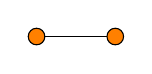
\begin{tikzpicture}
      \draw (3, 0) -- (4, 0);
      \foreach \x in {3,4} {
        \node [draw, fill=morange, circle, inner sep = 0, minimum size = 6] at (\x, 0) {};
      }
    \end{tikzpicture}
    \quad
    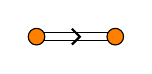
\begin{tikzpicture}
      \draw (0, 0.05) -- (1, 0.05);
      \draw (0, -0.05) -- (1, -0.05);

      \draw [thick] (0.45, 0.1) -- (0.55, 0) -- (0.45, -0.1);

      \foreach \x in {0,1} {
        \node [draw, fill=morange, circle, inner sep = 0, minimum size = 6] at (\x, 0) {};
      }
    \end{tikzpicture}
    \quad
    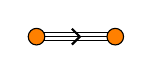
\begin{tikzpicture}
      \draw (0, 0.05) -- (1, 0.05);
      \draw (0, 0) -- (1, 0);
      \draw (0, -0.05) -- (1, -0.05);

      \draw [thick] (0.45, 0.1) -- (0.55, 0) -- (0.45, -0.1);

      \foreach \x in {0,1} {
        \node [draw, fill=morange, circle, inner sep = 0, minimum size = 6] at (\x, 0) {};
      }
    \end{tikzpicture}
  \end{center}
\end{eg}

The conditions on the matrices $A^{ij}$ now translate to conditions on the Dynkin diagrams, and it turns out we can classify all of them as follows:
\begin{thm}[Cartan classification]
  The possible Dynkin diagrams include the following infinite families (where $n$ is the number of vertices):
  \begin{center}
    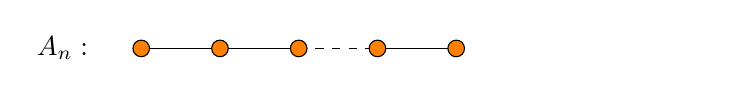
\begin{tikzpicture}
      \node at (-1, 0) {$A_n:$};
      \draw (0, 0) -- (2, 0);
      \draw [dashed] (2, 0) -- (3, 0);
      \draw (3, 0) -- (4, 0);
      \foreach \x in {0,1,2,3,4} {
        \node [draw, fill=morange, circle, inner sep = 0, minimum size = 6] at (\x, 0) {};
      }
      \node at (7, 0) {};
    \end{tikzpicture}
  \end{center}
  \begin{center}
    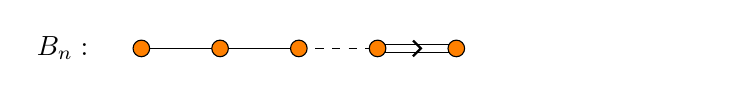
\begin{tikzpicture}
      \node at (-1, 0) {$B_n:$};
      \draw (0, 0) -- (2, 0);
      \draw [dashed] (2, 0) -- (3, 0);
      \draw (3, 0.05) -- (4, 0.05);
      \draw (3, -0.05) -- (4, -0.05);

      \draw [thick] (3.45, 0.1) -- (3.55, 0) -- (3.45, -0.1);

      \foreach \x in {0,1,2,3,4} {
        \node [draw, fill=morange, circle, inner sep = 0, minimum size = 6] at (\x, 0) {};
      }
      \node at (7, 0) {};
    \end{tikzpicture}
  \end{center}
  \begin{center}
    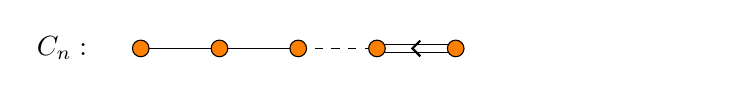
\begin{tikzpicture}
      \node at (-1, 0) {$C_n:$};
      \draw (0, 0) -- (2, 0);
      \draw [dashed] (2, 0) -- (3, 0);
      \draw (3, 0.05) -- (4, 0.05);
      \draw (3, -0.05) -- (4, -0.05);

      \draw [thick] (3.55, 0.1) -- (3.45, 0) -- (3.55, -0.1);

      \foreach \x in {0,1,2,3,4} {
        \node [draw, fill=morange, circle, inner sep = 0, minimum size = 6] at (\x, 0) {};
      }
      \node at (7, 0) {};
    \end{tikzpicture}
  \end{center}
  \begin{center}
    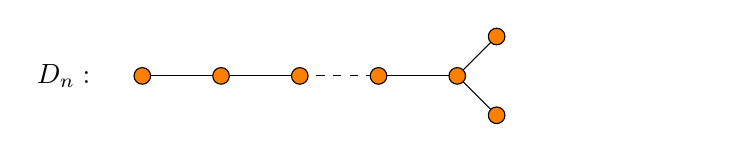
\begin{tikzpicture}
      \node at (-1, 0) {$D_n:$};
      \draw (0, 0) -- (2, 0);
      \draw [dashed] (2, 0) -- (3, 0);
      \draw (3, 0) -- (4, 0);
      \draw (4.5, 0.5) -- (4, 0) -- (4.5, -0.5);

      \foreach \x in {0,1,2,3,4} {
        \node [draw, fill=morange, circle, inner sep = 0, minimum size = 6] at (\x, 0) {};
      }
      \node [draw, fill=morange, circle, inner sep = 0, minimum size = 6] at (4.5, 0.5) {};
      \node [draw, fill=morange, circle, inner sep = 0, minimum size = 6] at (4.5, -0.5) {};
      \node at (7, 0) {};
    \end{tikzpicture}
  \end{center}
  And there are also five exceptional cases:
  \begin{center}
    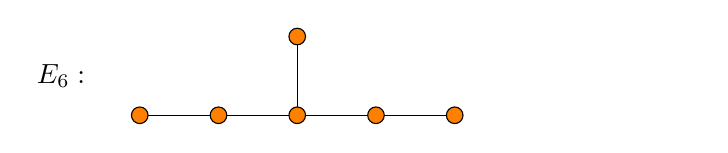
\begin{tikzpicture}
      \node at (-1, 0.5) {$E_6:$};
      \draw (0, 0) -- (4, 0);
      \draw (2, 0) -- (2, 1);
      \foreach \x in {0,1,2,3,4} {
        \node [draw, fill=morange, circle, inner sep = 0, minimum size = 6] at (\x, 0) {};
      }
      \node [draw, fill=morange, circle, inner sep = 0, minimum size = 6] at (2, 1) {};
      \node at (7, 0) {};
    \end{tikzpicture}
  \end{center}
  \begin{center}
    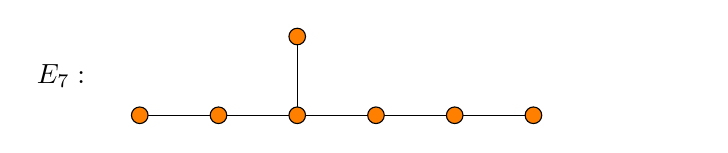
\begin{tikzpicture}
      \node at (-1, 0.5) {$E_7:$};
      \draw (0, 0) -- (5, 0);
      \draw (2, 0) -- (2, 1);
      \foreach \x in {0,1,2,3,4,5} {
        \node [draw, fill=morange, circle, inner sep = 0, minimum size = 6] at (\x, 0) {};
      }
      \node [draw, fill=morange, circle, inner sep = 0, minimum size = 6] at (2, 1) {};
      \node at (7, 0) {};
    \end{tikzpicture}
  \end{center}
  \begin{center}
    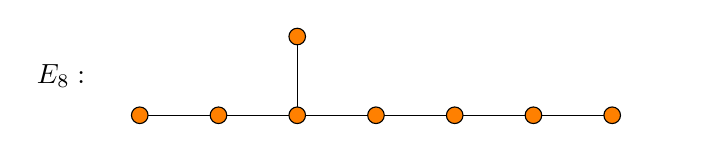
\begin{tikzpicture}
      \node at (-1, 0.5) {$E_8:$};
      \draw (0, 0) -- (6, 0);
      \draw (2, 0) -- (2, 1);
      \foreach \x in {0,1,2,3,4,5,6} {
        \node [draw, fill=morange, circle, inner sep = 0, minimum size = 6] at (\x, 0) {};
      }
      \node [draw, fill=morange, circle, inner sep = 0, minimum size = 6] at (2, 1) {};
      \node at (7, 0) {};
    \end{tikzpicture}
  \end{center}

  \begin{center}
    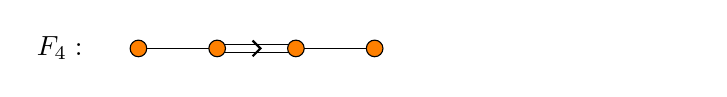
\begin{tikzpicture}
      \node at (-1, 0) {$F_4:$};
      \draw (0, 0) -- (1, 0);
      \draw (2, 0) -- (3, 0);

      \draw (1, 0.05) -- (2, 0.05);
      \draw (1, -0.05) -- (2, -0.05);

      \draw [thick] (1.45, 0.1) -- (1.55, 0) -- (1.45, -0.1);

      \foreach \x in {0,1,2,3} {
        \node [draw, fill=morange, circle, inner sep = 0, minimum size = 6] at (\x, 0) {};
      }
      \node at (7, 0) {};
    \end{tikzpicture}
  \end{center}
  \begin{center}
    \begin{tikzpicture}
      \node at (-1, 0) {$G_2:$};
      \draw (0, 0.05) -- (1, 0.05);
      \draw (0, 0) -- (1, 0);
      \draw (0, -0.05) -- (1, -0.05);

      \draw [thick] (0.45, 0.1) -- (0.55, 0) -- (0.45, -0.1);

      \foreach \x in {0,1} {
        \node [draw, fill=morange, circle, inner sep = 0, minimum size = 6] at (\x, 0) {};
      }
      \node at (7, 0) {};
    \end{tikzpicture}
  \end{center}
\end{thm}

\begin{eg}
  The infinite families $A_n, B_n, C_n, D_n$ correspond to well-known complex Lie groups by
  \begin{center}
    \begin{tabular}{cc}
      \toprule
      Family & Lie Group\\
      \midrule
      $A_n$ & $\mathcal{L}_\C(\SU(n + 1))$\\
      $B_n$ & $\mathcal{L}_\C(\SO(2n + 1))$\\
      $C_n$ & $\mathcal{L}_\C (\Sp(2n))$\\
      $D_n$ & $\mathcal{L}_\C (\SO(2n))$\\
      \bottomrule
    \end{tabular}
  \end{center}
  where the $\Sp(2n)$ are the \term{symplectic matrices}.
\end{eg}

Note that there is some repetition in our list. For example, we have $A_1 = B_1 = C_1 = D_1$ and $B_2 = C_2$. Also, $D_2$ is does not give a simple Lie algebra, since it is disconnected. We have $D_2 \cong A_1 \oplus A_1$. So we have
\[
  \mathcal{L}_\C(\SO(4)) \cong \mathcal{L}_\C(\SU(2)).
\]
Finally, we also have $D_3 = A_3$, and this reflects an isomorphism
\[
  \mathcal{L}_\C(\SU(4)) \cong \mathcal{L}_\C(\SO(6)).
\]
This classification is very important in modern theoretical physics, since in many theories, we need to pick a Lie group as, say, our gauge group. So knowing what Lie groups are around lets us know what theories we can have.

\subsection{Reconstruction}
Now given the Cartan matrix, we want to reconstruct the Lie algebra itself.

Recall that we had a Cartan-Weyl basis
\[
  \{H^i, E^\alpha: i = 1, \cdots, r: \alpha \in \Phi\}.
\]
The first thing to do in the reconstruction is to figure out what the set of roots are.

By definition, the Cartan matrix determines simple roots $\alpha_{(i)}$ for $i = 1, \cdots, r$. We can read off the inner products from the Cartan matrix as
\[
  A^{ij} = \frac{2(\alpha_{(i)}, \alpha_{(j)})}{(\alpha_{(j)}, \alpha_{(j)})} = \frac{2|\alpha_{(i)}|}{|\alpha_{(j)}|} \cos \varphi_{ij}.
\]
This allows us to find the simple roots.

How about the other roots? We can find them by considering the root strings, as we know that the length of the $\alpha_{(i)}$-string through $\alpha_{(j)}$ is given by
\[
  \ell_{ij} = 1 - A_{ji} \in \N.
\]
So we can work out the length of the root string from each simple root. By Cartan's theorem, this gives us all roots.

\begin{eg}
  Consider $\mathfrak{g} = A_2$. We have a Dynkin diagram
  \begin{center}
    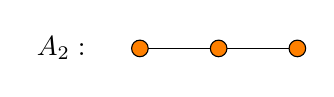
\begin{tikzpicture}
      \node at (-1, 0) {$A_2:$};
      \draw (0, 0) -- (2, 0);
      \foreach \x in {0,1,2} {
        \node [draw, fill=morange, circle, inner sep = 0, minimum size = 6] at (\x, 0) {};
      }
    \end{tikzpicture}
  \end{center}
  So we see that the Cartan matrix is
  \[
    A =
    \begin{pmatrix}
      2 & -1\\
      -1 & 2
    \end{pmatrix}.
  \]
  So we know that $\mathfrak{g}$ has two simple roots $\alpha, \beta \in \Phi$, and we know
  \[
    A_{12} = A_{21} = \frac{2(\alpha, \beta)}{(\alpha, \alpha)} = \frac{2(\beta, \alpha)}{(\beta, \beta)} = -1.
  \]
  So we find that $(\alpha, \alpha) = (\beta, \beta)$, and $\varphi_{\alpha\beta} = \frac{2\pi}{3}$. So we can display the roots as
  \begin{center}
    \begin{tikzpicture}
      \draw [->] (0, 0) -- (2, 0) node [right] {$\alpha$};
      \draw [->] (0, 0) -- (-1, 1.732) node [above] {$\beta$};
      \draw (0.6, 0) arc(0:120:0.6) node [pos=0.5, anchor=south west] {$\frac{2\pi}{3}$};
    \end{tikzpicture}
  \end{center}
  Since $\alpha, \beta \in \Phi_s$, we know $\pm(\alpha - \beta) \not\in \Phi$, and also we have
  \[
    \ell_{\alpha, \beta} = \ell_{\beta, \alpha} = 1 - \frac{2 (\alpha, \beta)}{(\alpha, \alpha)} = 2.
  \]
  So we have roots $\beta + n \alpha, \alpha + \tilde{n}\beta$ for $n, \tilde{n} \in \{0, 1\}$. So in fact our list of roots contain
  \[
    \alpha, \beta, \alpha + \beta \in \Phi.
  \]
  These are the positive. We know each of these roots has a negative counterpart. So we have more roots
  \[
    -\alpha, -\beta, -\alpha - \beta \in \Phi.
  \]
  Then by our theorem, we know these are all the roots. We can find the length of $\alpha + \beta$ by
  \begin{align*}
    (\alpha + \beta, \alpha + \beta) &= (\alpha, \alpha) + (\beta, \beta) + 2(\alpha, \beta)\\
    &= (\alpha, \alpha) + (\beta + \beta) - (\beta, \beta)\\
    &= (\alpha, \alpha).
  \end{align*}
  So in fact all roots have the same length. So if we draw all our roots, we get
  \begin{center}
    \begin{tikzpicture}
      \draw [->] (0, 0) -- (2, 0) node [right] {$\alpha$};
      \draw [->] (0, 0) -- (-1, 1.732) node [above] {$\beta$};
      \draw [->] (0, 0) -- (1, 1.732) node [right] {$\alpha + \beta$};
      \draw [->] (0, 0) -- (-2, 0) node [left] {$-\alpha$};
      \draw [->] (0, 0) -- (1, -1.732) node [below] {$-\beta$};
      \draw [->] (0, 0) -- (-1, -1.732) node [below] {$-\alpha - \beta$};
    \end{tikzpicture}
  \end{center}
  So the Cartan-Weyl basis consists of 
  \[
    \mathcal{B}_{\mathrm{CW}} = \{H^1, H^2, E^{\pm \alpha}, E^{\pm \beta}, E^{\pm(\alpha + \beta)}\}.
  \]
  This is the complete Cartan-Weyl basis of $A_2$. So this has dimension $2 + 6 = 8$.

  If we want to find out the brackets of these things, we look at the ones we have previously written down, and use the Jacobi identity many times.
\end{eg}

\section{Representation of Lie algebras}
Let $R$ be a representation of $\mathfrak{g}$ of dimension $N \in \N$. This is completely determined by the maps
\begin{align*}
  H^i &\mapsto \rho(H^i) \in \Mat_N(\C)\\
  E^\alpha &\mapsto \rho(H^\alpha) \in \Mat_N(\C)
\end{align*}
Here we need to make an assumption that the representatives $\rho(H^i)$ of the Cartan generators are diagonalizable. We then have
\[
  [\rho(H^i), \rho(H^j)] = \rho([H^i, H^j]) = 0
\]
for all $i$ and $j$. Since each of them are individually diagonalizable, we know that the $\rho(H^i)$ are simultaneously diagonalizable. So the representation space $V \cong \C^N$ is spanned by the simultaneous eigenvectors of $\{\rho(H^i)\}$. In other words, we can write
\[
  V = \bigoplus_{\lambda \in S_\rho} V_\lambda,
\]
where $V_\lambda$ is the eigenspace corresponding to eigenvalues $\lambda^1, \cdots, \lambda^r$, ie. for all $v \in V$, we have $\rho(H^i)v = \lambda^i v$.

The eigenvalue $\lambda \in \mathfrak{h}^*$ is a \term{weight} of $\rho$. The set $S_\lambda$ is called the \term{weight set} of the representation.

Note that the weights can have multiplicity, ie. $V_\lambda$ need not be $1$-dimensional. We write
\[
  m_\lambda = \dim V_\lambda \geq 1
\]
for the \term{multiplicity} of the weight.

By definition, we have
\[
  [H^i, E^\alpha] = \alpha^i E^\alpha
\]
So we have
\[
  \ad_H^i E^\alpha = \alpha^i E_\alpha.
\]
In terms of the adjoint representation, this says
\[
  \rho_{\mathrm{adj}} (H^i) E_\alpha = \alpha^i E_\alpha.
\]
So the roots $\alpha$ are the weights of the adjoint representation. We now want to figure out the allowed values of the weights.

Recall that for $\su_\C(2)$, we know that the weights are always integers. This will the case in general as well.

We start by consider the action of the step operator $\rho(E^\alpha)$ for $\alpha\in \Phi$ on $V_\lambda$. We let $v \in V_\lambda$. Then we have
\[
  \rho(H^i) \rho(E^\alpha)v = \rho(E^\alpha) \rho(H^i) v + [\rho(H^i), \rho(E^\alpha)] v.
\]
We know that
\[
  [\rho(H^i), \rho(E^\alpha)] = \rho([H^i, E^\alpha]) = \alpha^i \rho(E^\alpha).
\]
So we know that if $v \in V_\lambda$, then
\[
  \rho(H^i)\rho(E^\alpha)v = (\lambda^i + \alpha^i) \rho(E^\alpha) v.
\]
So the weight of the vector has been shifted by $\alpha$. Thus, for all vectors $v \in V_\lambda$, we find that
\[
  \rho(E^\alpha) v \in V_{\lambda + \alpha}.
\]
However, we do not know a priori if $V_{\lambda + \alpha}$ is a thing at all. $V_{\lambda + \alpha} = 0$, ie. $\lambda + \alpha$ is not a weight, then we know that $\rho(E^\alpha) v = 0$.

So the Cartan element $H^i$ preserve the weights, and the step operators $E^\alpha$ increment the weights by $\alpha$.

Consider the action of our favorite $\sl(2)_\alpha$ subgroup on the representation space. In other words, we consider the action of $\{\rho(h^\alpha), \rho(e^\alpha), \rho(e^{-\alpha})\}$ on $V$. Then $V$ becomes the representation space for some representation $\rho_\alpha$ for $\sl(2)_\alpha$.

Now we can use what we know about the representations of $\sl(2)$ to get something interesting about $V$. For any $v \in V_\lambda$, after some lines of algebra, we find that
\[
  \rho(h^\alpha)(v) = \frac{2(\alpha, \lambda)}{(\alpha, \alpha)} v.
\]
So we know that we must have
\[
  \frac{2(\alpha, \lambda)}{(\alpha, \alpha)} \in \Z
\]
for all $\lambda \in S_\rho$ and $\alpha \in \Phi$. This gives us a severe constraint on the possible forms of representations.
\printindex
\end{document}
